\documentclass[a4paper]{article}

\usepackage{preamble}
\begin{document}
% CREATED BY DAVID FRISK, 2015

% COVER PAGE
\begin{titlepage}
\newgeometry{top=3cm, bottom=3cm,
      left=2.25 cm, right=2.25cm} % Temporarily change margins

\pagenumbering{roman}
% Cover page background
%\AddToShipoutPicture*{\backgroundpic{-4}{56.7}{figure/frontpage_eng.png}}
\AddToShipoutPicture*{\backgroundpic{-80}{800}{figure/AvancezChalmersU_black_right.eps}}
\addtolength{\voffset}{2cm}
\vspace*{-1.75cm}
\rule{\linewidth}{1pt}


% Cover picture (replace with your own or delete)
%\begin{figure}[H]
%\centering
%\vspace{2cm}  % Adjust vertical spacing here
%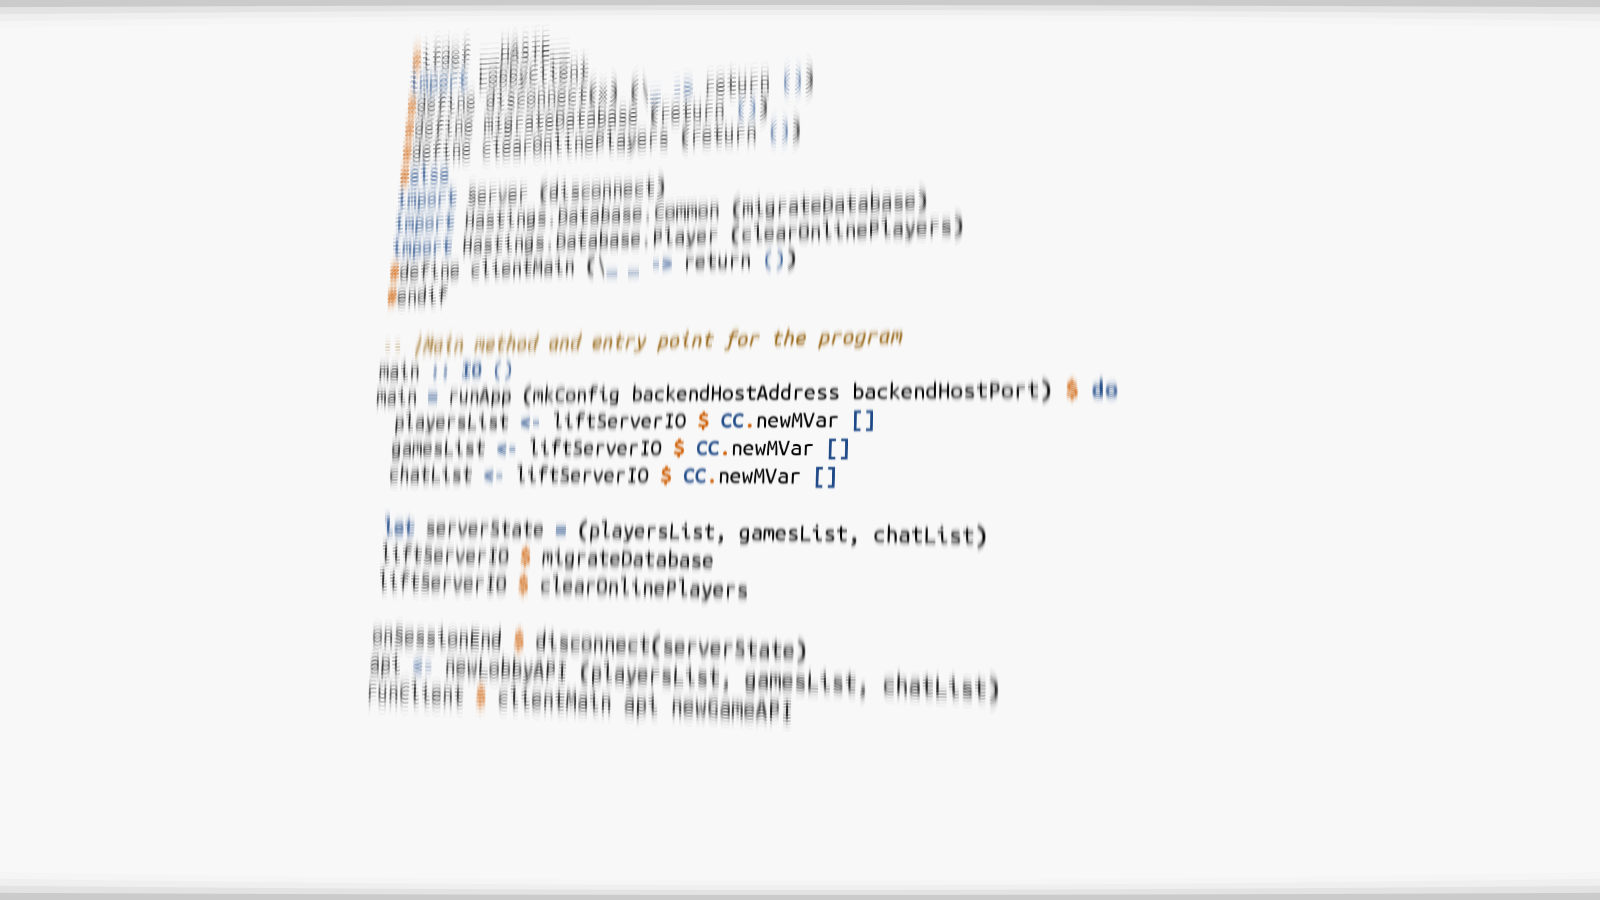
\includegraphics[width=0.9\linewidth]{title.png}
%\end{figure}


% Cover text
\mbox{}
\vfill
\renewcommand{\familydefault}{\sfdefault} \normalfont % Set cover page font
\textbf{{\huge Evaluating Haste.App: Haskell in a web setting}}   \\[0.5cm]
{\Large Effects of using a seamless, linear, client-centric programming model}\\[0.5cm]
Bachelor Science Thesis in Computer Science and Engineering \setlength{\parskip}{1cm}



{\Large \textsc{Benjamin Block}} \setlength{\parskip}{2.9cm}\\
{\Large \textsc{Joel Gustafsson}} \setlength{\parskip}{2.9cm}\\
{\Large \textsc{Michael Milakovic}} \setlength{\parskip}{2.9cm}\\
{\Large \textsc{Mattias Nilsen}} \setlength{\parskip}{2.9cm}\\
{\Large \textsc{André Samuelsson}} \setlength{\parskip}{2.9cm}

\vfill
\vspace*{-1.75cm}
\rule{\linewidth}{1pt}
Department of Computer Science and Engineering \\
\textsc{Chalmers University of Technology} \\
%\textsc{University of Gothenburg} \\
Gothenburg, Sweden, June 2016

\renewcommand{\familydefault}{\rmdefault} \normalfont % Reset standard font
\end{titlepage}
\restoregeometry
% TITLE PAGE
\newpage\null\thispagestyle{empty}\newpage

\newpage
\thispagestyle{empty}
\begin{center}
	\textsc{\large Bachelor of science thesis}\\[4cm]
	% Report number given by department 
	\textbf{\Large Evaluating Haste.App: Haskell in a web setting} \\[1cm]
	{\large Effects of using a seamless, linear, client-centric programming model}\\[1cm]
    {\Large \textsc{Benjamin Block}} \setlength{\parskip}{2.9cm}\\
    {\Large \textsc{Joel Gustafsson}} \setlength{\parskip}{2.9cm}\\
    {\Large \textsc{Michael Milakovic}} \setlength{\parskip}{2.9cm}\\
    {\Large \textsc{Mattias Nilsen}} \setlength{\parskip}{2.9cm}\\
    {\Large \textsc{André Samuelsson}} \setlength{\parskip}{2.9cm}
	
	\vfill	
	% Logotype on titlepage	
	\begin{figure}[H]
	\centering
	% Remove the following line to remove the titlepage logotype
	
\includegraphics[width=0.2\pdfpagewidth]{figure/logo_eng.pdf} \\	
	\end{figure}	\vspace{5mm}	
	
	Department of Computer Science and Engineering \\
	
	\textsc{Chalmers University of Technology} \\
	%\textsc{University of Gothenburg} \\
	Gothenburg, Sweden, June 2016 \\
\end{center}


% IMPRINT PAGE (BACK OF TITLE PAGE)
\newpage
\thispagestyle{plain}
%\vspace*{4.5cm}

\textbf{Evaluating Haste.App: Haskell in a web setting}\\
Effects of using a seamless, linear, client-centric programming model\\

{ \textsc{Benjamin Block}} \setlength{\parskip}{2.9cm}\\
{ \textsc{Joel Gustafsson}} \setlength{\parskip}{2.9cm}\\
{ \textsc{Michael Milakovic}} \setlength{\parskip}{2.9cm}\\
{ \textsc{Mattias Nilsen}} \setlength{\parskip}{2.9cm}\\
{ \textsc{André Samuelsson}} \setlength{\parskip}{2.9cm}

\copyright ~ Benjamin Block, 2016. \setlength{\parskip}{1cm}\\
\copyright ~ Joel Gustafsson, 2016. \setlength{\parskip}{1cm}\\
\copyright ~ Michael Milakovic, 2016. \setlength{\parskip}{1cm}\\
\copyright ~ Mattias Nilsen, 2016. \setlength{\parskip}{1cm}\\
\copyright ~ André Samuelsson, 2016. \setlength{\parskip}{1cm}

Supervisor: Emil Axelsson\\
Examiner: Niklas Broberg, Department of Computer Science and Engineering\setlength{\parskip}{1cm}

Chalmers University of Technology\\
%University of Gothenburg\\
Department of Computer Science and Engineering\\
SE-412 96 Gothenburg\\
Sweden\\
Telephone +46 31 772 1000 \setlength{\parskip}{0.5cm}

\vfill

The Authors grants to Chalmers University of Technology the non-exclusive right to publish the Work electronically and in a non-commercial purpose make it accessible on the Internet. The Author warrants that he/she is the author to the Work, and warrants that the Work does not contain text, pictures or other material that violates copyright law.

The Author shall, when transferring the rights of the Work to a third party (for example a publisher or a company), acknowledge the third party about this agreement. If the Author has signed a copyright agreement with a third party regarding the Work, the Author warrants hereby that he/she has obtained any necessary permission from this third party to let Chalmers University of Technology store the Work electronically and make it accessible on the Internet.

\vfill
% Caption for cover page figure if used, possibly with reference to further information in the report
%Cover: Wind visualization constructed in Matlab showing a surface of constant wind speed along with streamlines of the flow. \setlength{\parskip}{0.5cm}

Department of Computer Science and Engineering\\
Gothenburg, Sweden 2016


\normalsize



%\pagenumbering{gobble}
\vfill

\newpage
% CREATED BY DAVID FRISK, 2015
{\Large \textbf{Evaluating Haste.App: Haskell in a web setting}}\\
{\Large Effects of using a seamless, linear, client-centric programming model}\\
\\
{ \textsc{Benjamin Block}} \setlength{\parskip}{2.9cm}\\
{ \textsc{Joel Gustafsson}} \setlength{\parskip}{2.9cm}\\
{ \textsc{Michael Milakovic}} \setlength{\parskip}{2.9cm}\\
{ \textsc{Mattias Nilsen}} \setlength{\parskip}{2.9cm}\\
{ \textsc{André Samuelsson}} \setlength{\parskip}{2.9cm}\\
\textit{
Department of Computer Science and Engineering\\
Chalmers University of Technology \setlength{\parskip}{0.5cm} \\
%University of Gothenburg
\setlength{\parskip}{0cm}}\\\\
Bachelor of Science Thesis

\thispagestyle{plain}			% Supress header 
\setlength{\parskip}{1em}
\section*{Preface}
We would like to thank our supervisor Emil Axelsson for his invaluable support and guidance during this project. We would also like to thank Anton Ekblad, the primary developer of Haste and Haste.App, for answering our questions throughout the work.

\section*{Abstract}
In this paper, we evaluate Haste.App, a newly developed Haskell library for distributed web applications. Haste.App promises to deliver multiple ease of use factors in addition to allowing the static type checking of Haskell to be extended over the network. It also pairs with the Haste compiler which compiles Haskell code to JavaScript. We conclude that Haste.App is a promising library that allows real world distributed web applications to be written in Haskell with ease. The seamless, client-centric programming model also has positive effects on programmer productivity. There are, however, some issues that will need to be addressed with Haste.App: some way of making sure the JavaScript is updated when the server is, standardisation when it comes to project structure, and some convenient way of handling DOM. In order to reach this conclusion, we evaluate Haste.App primarily based on three key aspects: performance, stability, and programmer productivity. The evaluation is performed by creating a simple online multiplayer board game and an attached lobby system.


\vfill
\textbf{Keywords}:
Haskell, Haste.App, Haste, functional programming, web development.
\newpage


\section*{Sammandrag}
I denna rapport utvärderar vi det nyutvecklade Haskellbiblioteket Haste.App, som syftar till att underlätta implementeringen av distribuerade webbapplikationer. Haste.App gör det möjligt att utöka Haskells statiska typkontroll över nätverkskommunikation samt ger programmeraren tillgång till ett antal bekvämlighetsfaktorer. Utöver det, levereras Haste.App tillsammans med Haskell till JavaScript kompilatorn Haste. Vi kommer fram till att Haste.App är ett lovande bibliotek som enkelt tillåter webbapplikationer att skrivas i Haskell. Den sömlösa, klientcentrerade programmeringsmodellen som Haste.App erbjuder har också positiva effekter på programmerares produktivitet. Däremot finns det ett fåtal problem som behöver ses över: den kompilerade Javscript-koden måste bli uppdaterad när servern blir uppdaterad, det behövs standarder för struktur på projekt i Haste.App, samt ett mer effektivt sätt att hantera DOM-manipulation. Vi nådde denna slutsats genom att undersöka Haste.App ur tre synvinklar: prestanda, stabilitet samt programmerares produktivitet. Denna undersökning genomförs genom att implementera ett enkelt brädspel för flera spelare som en webbapplikation med ett tillhörande lobbysystem.
\vfill
\textbf{Nyckelord}:
Haskell, Haste.App, Haste, funktionell programmering, webbutveckling.


\newpage
\tableofcontents

\newpage

\glsaddall

\setglossarystyle{super}
\printnoidxglossary


\newpage
\pagenumbering{arabic}


\section{Introduction}
Haste.App is a new Haskell library for writing seamless client-server applications. The library addresses some of the prevailing issues with traditional web development. It allows the programmer to write a client-server application in a single file and extends type checking over the network. There are a lot of promising advantages with Haste.App and utilising functional programming when developing web applications.

\subsection{Background}
Writing interactive web applications typically involves JavaScript for a significant portion of the client-side code. The prevalence of JavaScript stems from the fact that it is supported by all significant web browsers and virtually all websites use some form of JavaScript \cite{flanagan2011javascript}. Because JavaScript is popular, it has a large community supporting it and a large number of libraries. Haskell, on the other hand, is not as popular as JavaScript but it has other benefits, such as its advanced type system. Other advantages include the ability to perform equational reasoning on the code \cite{gibbons2011just} and a powerful testing library called QuickCheck \cite{Claessen:2011:QLT:1988042.1988046}.

Haste is a Haskell to JavaScript compiler. It makes it possible to use the advantages of a pure functional language in a web setting. Haste is based on the Glasgow Haskell Compiler, and its primary aim is to produce compact JavaScript code \cite{a-distributed-haskell-for-the-modern-web}.

Haste is bundled with the library Haste.App which allows both the client- and server-side code to be written in one program \cite{ekblad2015seamless}. The library takes care of the network communication, alleviating the programmer from writing it explicitly. As such, the programmer is relieved from this tedious and error-prone task. Moreover, Haste.App is  pursuing a client-centric programming model, which means that the programmer writes the code from the client's perspective \cite{a-distributed-haskell-for-the-modern-web}. At the time of writing this thesis, Haste.App is still very new and requires more testing and investigation.

\subsection{Purpose}
\label{sec:purpose}
The purpose of this paper is to evaluate the advantages and disadvantages of writing client-server applications using the library Haste.App, with all of the properties of using a pure functional language. The language used is Haskell and Haste.App is an extension of the Haskell to JavaScript compiler Haste. Firstly, it is investigated whether or not there is any effect on performance, secondly, if there are any benefits regarding the stability of the application, and thirdly, if there are any advantages in regard to programmer productivity. An additional purpose of the project is to supply comments and feedback on Haste and Haste.App back to the developer, who is a Ph.D. student at Chalmers University of Technology.

\subsection{Limitations}
\label{sec:limitations}
The work does not assess demanding real-time applications and graphics with Haste.App since the focus of the project is mainly to evaluate the suitability of using Haste.App and Haskell to program for the web. Neither is a second application created using a more traditional library, for purposes of comparison. Furthermore, the usability \cite{usability} of programming in Haste.App is only considered on one point, namely by programmer productivity which is what is called efficiency in usability terms, the other parts are out of scope for this work. 

%\subsection{Related research}
%\todo{Remove.}
%There are two ways to view related research regarding this project. The first being a greater overview of functional research, particularly applied functional programming which Chalmers University of Technology is heavily pursuing. The research done in this thesis is another example of functional programming applied to an area where it is not so commonly used today, namely web development.

%The other view is research directly related to the work of this thesis. This thesis is related to the work of Anton Ekblad, who is the main developer of the Haste compiler and its accompanying libraries. In his licentiate thesis, "A Distributed Haskell for the Modern Web", he describes the implementation of Haste.App and its potential benefits \cite{a-distributed-haskell-for-the-modern-web}.

%Regarding general language $X$ to JavaScript compilers, there is also much research. Many programming languages have a JavaScript compiler; an example is ClojureScript which is a Clojure to JavaScript compiler \cite{clojure-ieee}.

\newpage
\section{Problem description}
\label{sec:problem}
The purpose of this paper is analysed by splitting it into several smaller parts. These deal with different aspects of writing client-server applications with the help of Haste.App. As mentioned in \cref{sec:purpose} the purpose can be split into effects on performance, stability and programmer productivity. These are, however, also large and hard to analyse without further breaking them into even smaller parts.


\subsection{Performance description}
\label{sub:performance-description}
Performance is a crucial aspect when writing client-server applications, and therefore a crucial aspect when assessing Haste.App. On the server-side, the application created with Haste.App can not be too demanding regarding system resources. This is important both because it is often desirable to have as inexpensive servers as possible (while maintaining enough performance), and because it allows more clients to be connected to the server. On the client-side, the application and code generated by Haste need to be efficient for the user's computer to run smoothly and to not experience any delays from performance issues. As such it is important that there is not a significant discrepancy between using Haste.App and a more traditional client-server approach. 

There could be several reasons for a significant divergence: firstly, on the client-side, the Haste compiler might generate JavaScript that is slower than equivalent JavaScript written directly in the language. Secondly, the server part of an application written in Haste.App must not be considerably slower than writing an application using a different library. 

\subsection{Stability description}
On a language level, Haskell brings many benefits to the stability of an application, as it is a strongly typed static language. The static type checking verifies type correctness at compile time which allows bugs which are trivial but hard to find to be tracked down more easily. Another important benefit the type system in Haskell brings is that it allows for pure logic to be separated from its impure counterparts. This type system brings a benefit by allowing the use of tools like QuickCheck to test the pure logic of the application \cite{Claessen:2011:QLT:1988042.1988046}. Haste.App also extends the static type checking over the network through its remote procedure calls (RPC), which might remove confusing network errors. 

The programmer can use these benefits when writing code for Haste.App. Stability is thus investigated in order to see if the advantages Haskell brings, in terms of program correctness, is of any practical use when writing client-server applications.

Besides language level correctness, the stability of the Haste compiler needs to be taken into account. Particularly the Haste.App module, which this project primarily focuses on, has to be evaluated to detect any errors. While these errors might decrease the stability of the application, they are not the fault of the program itself. This is where giving feedback on Haste and Haste.App becomes important as it allows bugs to be tracked down and fixed.


\subsection{Programmer productivity description}
\label{sec:programmer_productivity}
Traditional client-server applications, in contrast to Haste.App, force the programmer to write two separate applications and the communication between them. Writing two applications can be an error-prone and tedious task as it forces the programmer to make sure the type of the data sent between the client and server match. Moreover, the arbitrary communication pattern can make the program flow confusing and difficult to grasp as well as introduce errors. In this traditional model, both the server and client can drive the program flow, something that also serves to make the program flow unpredictable. These are all problems when considering programmer productivity.

Haste.App tries to counter these issues in a number of ways. Most importantly it allows the programmer to write both the client code and the server code in the same file and makes use of Haskell's strong and static type checking to handle the communication. It also lets the client be the only driving force in the application and uses a synchronous, linear programming model \cite{ekblad2015seamless}. Furthermore, Haskell has been shown to have some ease-of-use aspects compared to imperative languages, such as not having to consider statement sequence,  \cite{mathematical-comparison-haskell-c++}. These ease-of-use aspects may influence programmer productivity. 



\newpage
\section{Technical background}
Developing a web application using Haskell and Haste.App requires the use of a number of technical tools, languages, and standards. What follows is a description of these tools, languages, and standards.


\subsection{Haskell}
Haskell is a pure functional language with static typing and lazy evaluation. In a pure functional language it is possible to separate functions with side-effects, such as writing to file or user input, from functions which only depend on the parameters given to that function. Moreover, Haskell is a statically typed language and offers compact syntax.


Handling side effects, or more generally computational contexts, is done by using monads. For programmers unfamiliar with the concept, it might seem like an unnecessary obstacle which is a byproduct of the language being fully functional. There are, however, many benefits of using monads, one being that it affects the type system in a positive way. Because monads are explicitly seen in the type system, the programmer can at a glance see which code runs in what computational context. 

Being a statically typed language means that all types are resolved at compile time instead of run time as it would have in a dynamically typed language. Static type checking brings benefits, mainly that trivial bugs can be caught at compile time. Knowing types at compile time also allows the compiler to do various optimisations otherwise not possible. The size of the compiled binaries also tends to become smaller and run more quickly because the code for checking types during run time can be omitted.

Haskell also offers very compact syntax, which may allow complex code to be expressed clearly. The clarity and reduced size of Haskell code can make it easier to digest functionality when reading new code. There is data supporting the fact that Haskell programs tend to be a lot more concise and smaller than object-oriented and imperative programs \cite{hudak1994haskell}. In addition, there exists a proportional relationship between the number of bugs and lines of code, generally independent of what language is used \cite{mcconnell2004code}. The brevity of Haskell and the relationship between lines of code and bugs could mean that an experienced programmer is more productive in a functional language than in an imperative one, if a programmer spends less time writing Haskell code than debugging.

\subsection{JavaScript}
\label{sec:javascript}
JavaScript is a high-level, dynamic and interpreted language which is standardised by the EcmaScript specification \cite{flanagan2011javascript}. Furthermore, it is supported by all major web browsers that are used today; this has made JavaScript a very popular language. However, despite its popularity, JavaScript still has several shortcomings. According to Ekblad, JavaScript suffers from several problems, including bad scoping semantics, weak typing, and poor support for the functional paradigm \cite{ekblad2012towards}. 

\subsection{Haste}
Haste is a Haskell to EcmaScript compiler developed by Anton Ekblad, a Ph.D. student at Chalmers University of Technology. The output from Haste will be referred to as JavaScript in this work since the most common implementation of EcmaScript is JavaScript as described in \cref{sec:javascript}. Haste is based on the Glasgow Haskell Compiler (GHC) because the bulk of the work that goes into improving the Haskell language is implemented in GHC \cite{ghc-compiler}. GHC also includes many language extensions that are widely used today \cite{ekblad2015seamless}. Because Haste utilise GHC, it can make use of almost all of the optimisations the GHC makes to Haskell code before converting the code to JavaScript. In addition, Haste is integrated with the Google Closure Compiler. The Google Closure Compiler is a JavaScript-to-JavaScript compiler that minimises and optimises the code \cite{google-closure}.

One of the primary aims for the Haste compiler is to produce lightweight and optimised code. Because of this, Haste does not support everything the GHC compiler does. Instead, Haste makes some compromises in order to perform optimisations of the generated code \cite{ekblad2015seamless}.

\subsection{Haste.App}
Haste.App is a library compatible with the Haste compiler used for writing client-server applications. There are several properties that make Haste.App different in comparison to the traditional way of writing network applications. 

Probably the most notable difference is that both the client and server logic is written in the same program. This allows for an extension of the powerful type system over the network. Haste.App makes it possible at compile time to verify that the type of data the client or server send and receive are correct. It is also easier to move functionality from the client to the server and vice versa.

Another significant feature of Haste.App is the abstraction of network communication. The programmer does not have to explicitly write the communication between the client and server. Instead of calling a function to send data over the network, the client can call the function on the server directly using special constructs, a combination of the \textit{remote} and \textit{onServer} functions. Functions that are called over the network in this way are always synchronous, which means that the client will wait for a response from the server before continuing the execution of the program. The abstraction of network communication is implemented using HTML5 WebSockets in Haste.App \cite{a-distributed-haskell-for-the-modern-web}.

Having all the logic in one program might seem to blur the distinction between the code executed on the client or server, but a separation is achieved using the Haskell type system. The code that is only executed on the server is wrapped in the \textit{Server} monad and the client code is wrapped in the \textit{Client} monad. Both monads are instances of the \textit{IO} monad. 

Uniting the client and server code also requires a different way of compiling the program. The code is first compiled with GHC, which generates the binary that is executed on the server. After GHC is done, the code is compiled with Haste which produces the JavaScript code that runs on the client. 

A simple example of Haste.App can be seen in \cref{fig:haste-app-example}. The \textit{main} function starts the app by creating a list variable containing names of the connected clients, wrapped in a \textit{MVar}, which is used as the server state. The \textit{MVar} (a synchronous variable) is lifted, i.e. has its context changed, into the Server context which tells Haste.App that it should only be available on the server. Also, in the main function the \textit{connect} and \textit{countClients} functions are wrapped in a remote context to enable them as remote procedural calls (RPCs). Being remote means that the function exists on the server but can be accessed by the client through a \textit{onServer} call. Following the creation of the remote function the client code begins, it prompts the client for a name and calls the \textit{remoteConnect} to add the acquired name to the servers state. It then calls the \textit{remoteCountClients} function and receives the number of connected players which is displayed to the client. 
\begin{figure}[H]
    \centering  
\begin{lstlisting}  
-- Entry point for both the Server and Client.
main = runApp defaultConfig $ do
  -- Mvar is a synchronized variable.
   clients <- liftServerIO $ newMVar []

   -- Create the remote functions which the
   --   client can call and execute on the server.
   remoteConnect <- remote $ connect clients
   remoteCountClients <- remote $ countClients clients

    -- Here client only code begins.
   runClient $ do
      name <- prompt "Hello! Name please!"
      -- <.> applies name as parameter to the remote function.
      onServer $ remoteConnect <.> name
      nbrOfClients <- onServer $ remoteCountClients
      alert ("Hello number " ++ show nbrOfClients)

-- | Add clients nick to server state i.e. the list of names.
connect :: Server (MVar [String]) -> String -> Server ()
connect remoteClientList name = do
  clients <- remoteClientList
  liftIO . modifyMVar_ clients $ \cs -> return $ name : cs

-- | Count the total number of clients connected.
countClients :: Server (MVar [String]) -> Server Int
countClients remoteClients = do
  clients <- remoteClients
  clientList <- liftIO $ readMVar clients
  return $ length clientList
\end{lstlisting}
    \caption{Simple Haste.App example that stores your name on the server and displays how many clients have entered to the connecting client.}
    \label{fig:haste-app-example}
\end{figure}

\subsection{DOM}
DOM or Document Object Model is a standard for representing documents that contain some markup languages, such as HTML. It allows for HTML pages to be written in a hierarchical tree-like manner and it allows for programs to interact with the contents of the page to create interactive websites. HTML, or HyperText Markup Language, is the standard for creating web pages.

The DOM in the form of HTML can be created in various ways. One approach is to use a separate file where raw HTML is accepted. Another approach is using JavaScript, or Haste in the case of this project, to create HTML elements and add them to the DOM tree. Another approach is to use an external library created for use with Haste. 

\subsection{SQL \& MySQL}
Structured Query Language (SQL) is a domain specific language designed to interact with a relational database management system (RDMS). In an RDMS data is stored in tables where each table is organised into columns and rows. Columns represent which type of data may be retained in the table and the list of rows represent the data stored in the table. MySQL is an open source implementation of most parts of the SQL standard. Its main features are the ability to handle large amounts of data and that it is relatively easy to setup \cite{mysql-features}. Databases are an important aspect of web development.

\newpage
\section{Method}
\label{sec:method}
To reach a conclusion regarding the purpose of the project a number of methodologies of evaluating performance, programmer productivity, and stability have been used. An application was written with Haste.App to enable data gathering from measurements and tests. Specifically, a lobby system for games was developed together with an implementation of the game Chinese Chequers. Further evaluation was based on observations and tests performed during or after the creation of the application. How the assessment of these areas of interest was done is discussed in more detail below. 


\subsection{How to measure performance}
\label{sub:method-performance}
Several different aspects needed to be taken into account to assess the overall performance of the application. Most notably, the speed of the application was measured. Because the application is hosted on a web page, there were primarily two metrics to be considered when measuring its speed. The amount of bandwidth sent between the server and the client and how much system resources were used by the application. The different methods used to measure system resources on the client and the server are explored below.

The bandwidth needed by the application was divided into two parts, the bandwidth required to transfer the JavaScript to the client from the server, and the bandwidth required when a client is using the application. This data was compared to other sites offering similar content to assess if the application requires a reasonable amount of bandwidth for what it does. Measuring the initial bandwidth was done by measuring the size of the generated JavaScript. Moreover, the bandwidth required during the connection was measured via \textit{Wireshark} \cite{wireshark-website}, a tool for monitoring network traffic.

The system resources used by the application on the server-side are defined by the CPU-usage, load average, network utilisation, and the amount of RAM required. To monitor these values the resource monitoring tool \textit{munin} \cite{munin-website} was used. On the client-side, on the other hand, performance was measured by looking at the total CPU time used by the executed JavaScript. The web browser Chrome was used together with its built-in developer tools to measure the total CPU time.

To test the performance of the server when there are many clients connected and interacting with the website, scripts were written with the help of the Ruby library \textit{Watir} \cite{watir-test-framework}. The library enabled a script to interact with the DOM elements of a web page. \textit{Watir} made it possible to simulate connected clients and simultaneously monitor and quantify CPU and memory usage on the server when a number of clients were connected.

\subsection{How to measure stability}
\label{sub:method-stability}
To measure the stability of the developed application, it was decided that a number of states should be monitored to make sure they were resistant to unrecoverable errors. An unrecoverable error is an error that cannot be handled by the application and forces a reset of the application state. The states were: 
\begin{enumerate}[noitemsep]
    \item When the server gets updated/restarted during an active session.
    \item If the client has outdated JavaScript when trying to communicate with the server.
    \item Runtime errors on the server.
    \item Runtime errors in the clients JavaScript.\\
\end{enumerate}

The first state was decided to be monitored as it is common that an update has to be made to the server. Preferably it should be possible to perform such an update without the user noticing a reconnection of the web socket. It could also be the case that the server crashes. In the event of such a crash, it would be preferable if the server could restart without the clients noticing the crash.

The second state was monitored since the source code is compiled twice, once with Haste and once with GHC. It could be easy to accidentally update only one of the two compiled sources. When this happens, either the client or the server can receive an unexpected value and may crash.

The third state was considered because Haste.App can potentially cause crashes on its own as it is a new library. Since it is a new library, it was important to measure if these issues were a problem. While crashes can occur based upon logical errors, such crashes were not taken into account. 

The final state was also considered since Haste is a relatively new library. Once again, what was primarily considered are crashes caused by Haste.App or Haste, since logical errors will be present regardless of the library. In the client JavaScript, however, there is another dimension compared to runtime errors on the server since the JavaScript is compiled with the Haste compiler. 



\subsection{How to measure programmer productivity}
\label{sub:method-programmer-productivity}
Assessing the programmer productivity of using Haste.App was difficult. Initially, it might seem like a very subjective criterion, and it partly is, but there were further aspects taken into account when measuring programmer productivity. What was considered were, errors present in Haste and Haste.App, possible effects of the client-centric and linear programming model of Haste.App, if the strong static type system of Haskell has any effects, and comparing the lines of code with other similar applications.

Looking at errors present in Haste and Haste.App was an important aspect. Since Haste is on version 0.5.4 during writing, there may be some prominent issues in both Haste and Haste.App, which would have to be worked around during development. They would be detrimental to programmer productivity.

The client-centric and linear programming model of Haste.App is another interesting aspect. Since this programming model differs to traditional web development \cite{ekblad2015seamless}, it was an important aspect to assess. The developer of Haste.App claims that this programming model can make the program flow easier to grasp \cite{ekblad2015seamless}. Therefore, it would have a positive effect on programmer productivity.

Moreover, programmer productivity can also be affected by the strong static type system of Haskell. The type system is considered in respect to if the number of hard-to-find errors in the code is reduced. Since Haste.App also allows Haskell's type system to be extended over the network communication, aspects regarding errors in network communication are also considered. 

Finally, the development of the application in this project was compared to other similar applications. Other applications were examined because difference in programmer productivity can be influenced by the number of lines of code required for that implementation. Lines of code in a project is an important aspect since it affects the maintainability as well as the development time.  

\subsection{An application to measure Haste.App}
To accurately assess Haste.App an application was developed in two parts, a lobby system and a game. These two parts were chosen because they could be used to look at different areas of the problems described in \cref{sec:problem}. What follows is a brief description of the different parts as well as what problems they illustrate.

\subsubsection{The Lobby system}
The lobby system enables connected clients to start conversations with each other and create their own session of the game. When creating a new game session other clients are able to join until the game is full or until the creator starts the game, thus enabling games to be played.

A lobby system was created to assess scalability and performance of Haste.App. The scalability and performance was to be tested through the lobby since it does not have an upper limit of connected clients or concurrently active games. The aim was to find, if it exists, a correlation between performance and connected clients. Another important benefit of developing a lobby system was to enable thorough testing of programmer productivity when working with Haste.App since it would be possible to test various libraries for common web development purposes.

\subsubsection{Chinese Chequers}
\label{sub:chinesecheckers}
To test more of the performance and continuous communication between clients aspects of Haste.App a board game was implemented. Chinese Chequers was chosen for its simplicity since Haste.App might not yet be suitable for dealing with demanding real-time applications.

Chinese Chequers is a turn-based board game available for two, four or six players. The rules are fairly simple. Each player is assigned pieces of one colour. In order to win, a player has to move all pieces of the player's colour to the opposite side of the board. The six moves a player can make are moving horizontally down or up to the left or right, or vertically. A player may only move their piece to either one of those positions if they are empty. In case a position that can be moved to is occupied, it can be jumped over. An example is shown in \cref{fig:chequers-move}. Jumping over a piece makes the player eligible to move the same piece by jumping over another piece again.
\begin{figure}[ht]
    \centering
    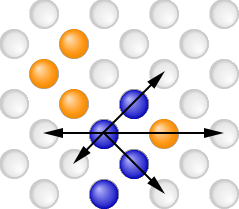
\includegraphics[width=0.3\textwidth]{figure/moves}
    \caption{Shows all the possible moves the blue chequer can do.}
    \label{fig:chequers-move}
\end{figure}

\newpage
\section{Development}
Developing an application in Haste.App may differ somewhat from the development of an application in a different programming model. Therefore, the process of developing an application using Haste.App is here described. The process of development was split into two parts: the game and the lobby system, which were developed in parallel. This section describes how the development was performed and crucial decisions which had to be made along with other important issues that had to be solved.

\subsection{Dependency management using Haste.App}
\label{sub:dependencies}
Since an application in Haste.App is compiled using two compilers, GHC and Haste; this presents some problems when using some external libraries as Haste does not support everything GHC supports. To solve this problem, conditional compilation was used, which enables the programmer to tell the compiler to ignore certain parts of the code when compiling with a specific compiler. An example of how this was done is shown in \cref{fig:dependencies-definitions}.

\begin{figure}[ht!]
\begin{lstlisting}
#ifdef __HASTE__
import LobbyClient
#define disconnect(x) (\_ -> return ())
#else
import LobbyServer
#define clientMain (\_ -> return ())
#endif
\end{lstlisting}
\caption{Definitions made to work around dependency problems.}
\label{fig:dependencies-definitions}
\end{figure}

In \cref{fig:dependencies-definitions} it is stated that if '\_\_HASTE\_\_' is defined i.e. the code is compiled by the Haste compiler, import \textit{LobbyClient}, but also make a dummy definition of the \textit{disconnect} function, since the actual disconnect function is defined in \textit{LobbyServer}. Likewise, if '\_\_HASTE\_\_' is not defined i.e. GHC is compiling, import only \textit{LobbyServer} and make a dummy definition of the \textit{clientMain}.

In general, if a Haskell library which Haste cannot compile is desired to be utilised on the client-side then the server needs to provide it through a remote function and return it in some data type which Haste can handle.

\subsection{Updating the client}
\label{sub:updating-client}
During the development, there was a problem with updating the client when a state change occurred. For example, when a client connects to the server all other clients should be notified. Since Haste.App is client-centric, the client has to be the one to initiate communication with the server. Two methods were considered to solve this problem. The first method works by reading a state from the server and then updating every couple of seconds. The second method instead uses a synchronous channel at the server. The server writes to the channel when an update occurs and the client reads from the channel continuously.

The first method, reading a state from the server, is more intuitive to construct than the second. It is also in line with the client-centric model of Haste.App, which makes the program flow easy to understand. However, this method drains additional resources as the client has a process reading the state of the server every couple of seconds. Upon reading the state, the process has to determine if the state has changed and then update accordingly. The method is illustrated in \cref{fig:reading-state}.

\begin{figure}[ht!]

\begin{subfigure}[]{\textwidth}
\begin{lstlisting}[language=Haskell]
-- Waits for an update in state to occur and then updates if it has
listenForUpdates :: State -> (State -> Client ()) -> Client ()
listenForUpdates oldState callback = do
    newState <- onServer readState
    if oldState == newState 
        then do
            -- if nothing has changed, wait a second before checking again
            setTimeout 1000 $ listenForUpdates oldState callback
        else do
            callback newState -- Update the client in some way
            listenForUpdates newState callBack
\end{lstlisting}
\subcaption{Client code, reads the state and then updates if it has changed}
\end{subfigure}

\begin{subfigure}[]{\textwidth}
\begin{lstlisting}[language=Haskell]
-- Simply reads the server state belonging to that client
readState :: StateList -> Server State
readState states = do
    sid <- getSessionID -- gets the unique session id
    liftIO $ do
        case sid `lookup` states of
            Nothing -> return emptyState -- "should not happen"
            Just state -> return state
    
\end{lstlisting}
\subcaption{Server code, returns the state}
\end{subfigure}
\caption{The method of reading a state from the server and then deciding if to update.}
\label{fig:reading-state}
\end{figure}
The second method, reading a synchronous channel, solves the problem with consuming resources that the first method has. This method is, however, more complicated in its construction. Since the channels are created and kept by the server, there has to be a function on the server for reading the channel. Reading from the channel is a blocking operation so there is, for each channel, a process waiting to read. Upon reading a value from a channel, through a remote call to the server, the client has to react to the message in some way. This method is illustrated in \cref{fig:reading-channel}. After careful consideration, this approach was decided to be used to communicate state changes in both the game and the lobby.

\begin{figure}[ht!]

\begin{subfigure}[]{\textwidth}
\begin{lstlisting}[language=Haskell]
-- Client-side method for reading a message from the server
listenForMessages :: Remote (Server Message) -> (Message -> Client ()) -> Client ()
listenForMessages serverReadChannel callBack = do
    msg <- onServer serverReadChannel -- call the server with the readChannel function
    callBack msg -- React to the read message in some way
                 -- Perhaps by getting a new state
    listenForChatMessages callBack -- recurse indefinitely
\end{lstlisting}
\subcaption{Reads the channel (at the server) and then reacts to the message, maybe by getting new state.}
\end{subfigure}

\begin{subfigure}[]{\textwidth}
\begin{lstlisting}[language=Haskell]
-- Called by a client to read its channel
readChannel :: Server (MVar [a]) -> Server Message
readChannel remoteClientChannels = do
    sid <- getSessionID -- gets the unique session id
    mVarClientChannels <- remoteClientChannels
    liftIO $ do
        clientList <- readMVar mVarClientChannels
        case sid `lookup` clientList of
            Nothing            -> return $ ErrorMessage "Couldn't find client."
            Just clientChannel -> readChan clientChannel -- readChan is blocking
\end{lstlisting}
\subcaption{Reads the client's state, if it can be found.}
\end{subfigure}

\caption{The method of reading a synchronous channel.}
\label{fig:reading-channel}
\end{figure}


\subsection{Development of the game}
\label{sec:game-development}
This section describes the rule set that was implemented in the game and the technical implementation. It also illustrates the choices taken during the development of the game sequentially.

\subsubsection{Implementation of the game rules}
\label{sec:game-rules}
The diagram in \cref{fig:flowchartGame} describes the actions a player can make. After a jump the game automatically moves to the next player but when a double jump (a jump over a chequer) is made it is possible to move again as seen in the flowchart, but only with the same chequer. In this implementation of the game, it is also possible to rotate the current player without moving a chequer. 
\begin{figure}[ht!]
    \centering
    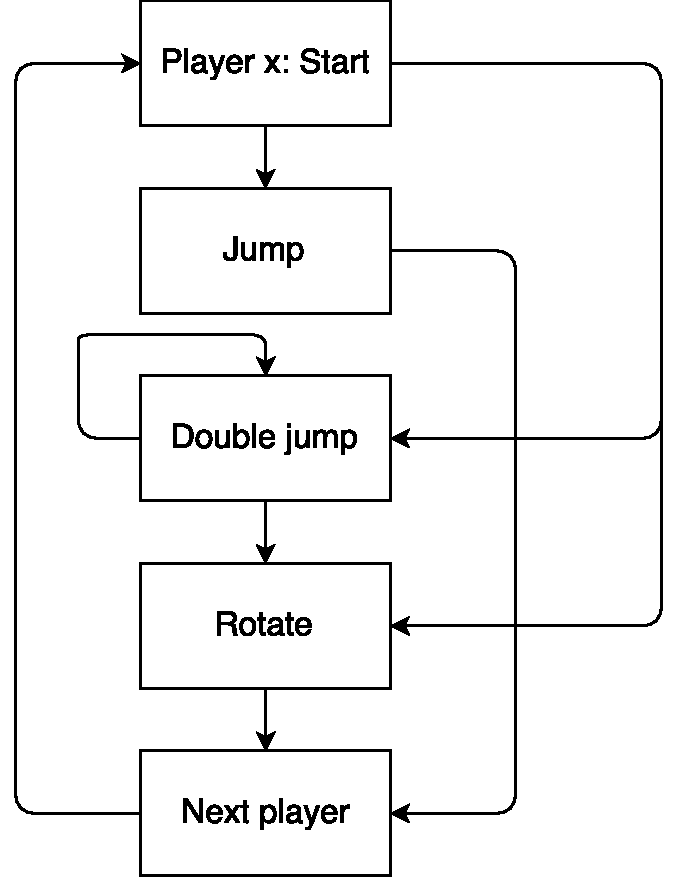
\includegraphics[scale=0.1,width=0.4\textwidth]{figure/flowchartGame}
    \caption{Displaying all possible actions a player can make within the game.}
    \label{fig:flowchartGame}
\end{figure}

\subsubsection{Game logic and data types}

The \cref{fig:gameTypes} illustrates the hierarchy in which the types depend on each other together with their definitions. The $Content$ data type was created to represent what every position can hold: it is either $Empty$ or it has a coloured piece, which is represented by the data constructor $Piece$ $Color$. The next crucial data type is $Square$. $Square$ is a product type containing a: $Color$, $Content$ and $Coord$. The $Coord$ type is simply a type synonym for $(Int,Int)$, representing the game logic coordinates. With the help of these types, the game table could be defined and it is represented by the $Table$ type. $Table$ is also a type synonym for $[Square]$. 

\begin{figure}[ht!]
    \centering
\begin{subfigure}{\textwidth}
    \centering
    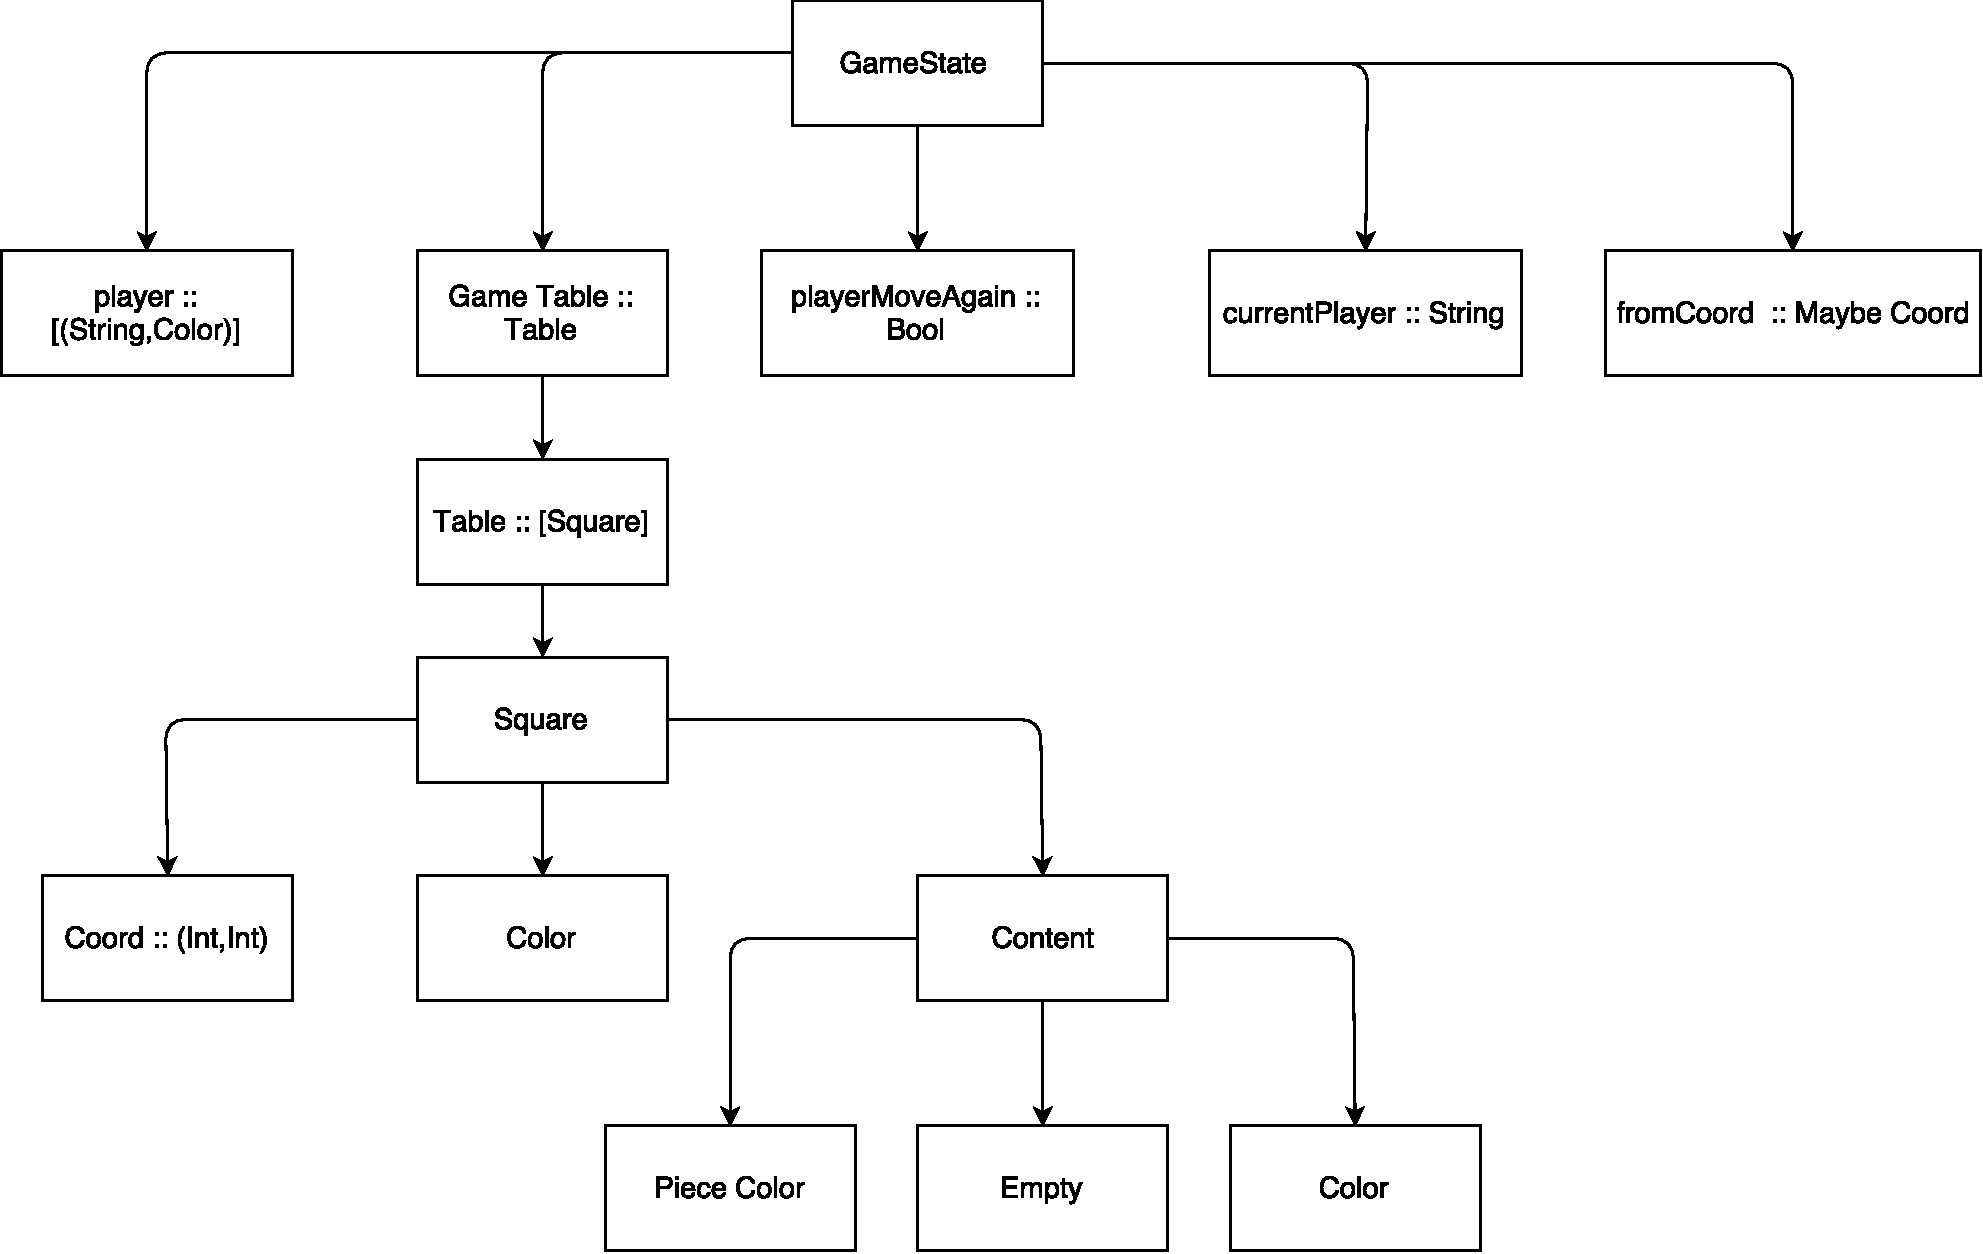
\includegraphics[scale=0.8,width=0.8\textwidth]{figure/gameTypesHierarchy}
    \caption{Visualisation of the game data types hierarchy. The root of the tree is the \textit{GameState}.}
\end{subfigure}
~
\begin{subfigure}{\textwidth}
\begin{lstlisting}
data Content = Empty | Piece Color

data Square = Square Content Color Coord

type Coord = (Int,Int)

type Table = [Square]

type Player = String

data GameState = GameState { players         :: [(String,Color)]
                           , gameTable       :: Table
                           , playerMoveAgain :: Bool }
                           , currentPlayer   :: String
                           , fromCoord       :: Maybe Coord
\end{lstlisting}
    \caption{The Haskell data types that are used in the game}
    \end{subfigure}
    \caption{Illustration of the data types that are used in the game}
    \label{fig:gameTypes}
\end{figure}


Furthermore, a way to represent the current state of the game was needed, and therefore, the $GameState$ type was created. $GameState$ contains the following: 
\begin{itemize}
    \item A $Table$ holding the current game table.
    \item The field $Players$ which is of type $[(Player,Color)]$ containing all the active players with their respective colour implemented as a regular queue.
    \item $CurrentPlayer$ is defined as a $Player$ which is a type synonym for a $String$.
    \item $MoveAgain$ which is of type $Bool$ used for checking if the current player can move again.
    
\end{itemize}
The $GameState$ is thus holding all information about a game session and is the root of the type tree in \cref{fig:gameTypes}. Each client stores their $GameState$ locally in an $MVar$.


\subsubsection{Graphical implementation}
\label{sec:graphimpl}

\begin{figure}[ht!]
    \centering
    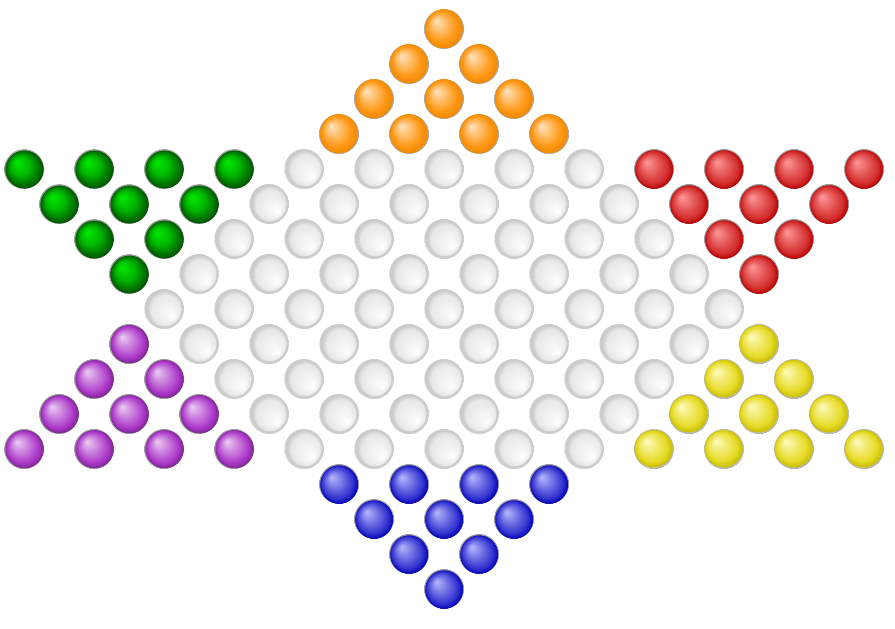
\includegraphics[scale=0.8,width=0.6\textwidth]{figure/game}
    \caption{The resulting game graphics.}
    \label{fig:gameGraphics}
\end{figure}


Haste provides a library for drawing and filling regular geometrical figures, but using these functions only achieves a pretty outdated graphical look. A decision was made to use bitmaps, which are just pictures that can be rendered on the screen. This gives a more modern graphical look, as seen in \cref{fig:gameGraphics}. 
Furthermore, a highlighting effect was achieved by changing the contrast and brightness of the bitmaps used to represent the chequers.

Upon clicking on the screen to interact with the game, the input coordinates need to be parsed to represent game logic coordinates. There were issues with generating the correct input coordinates when using the function supplied with Haste. To solve the coordinates issue, the FFI for getting the game board position on the screen was needed. The FFI is used to call JavaScript directly from Haskell. Knowing the game board position and the current scrolled offset on the page, the correct input coordinates could be calculated. 


\subsubsection{Network communication}
The first approach to communication between the client and server was to let the server give each client channels, from Haskell's $Control.Concurrent$ package. They did not work with Haste, which seemed strange since the $MVars$ from $Control.Concurrent$ had been used without a flaw.

The issue regarding the channels was solved by only reading and writing to the channels on server-side. The client simply requests the server to read or write to the channels located on the server. Using the channels from $Control.Concurrent$ works on server-side since the code is only compiled with GHC. Updating the client is described in more detail in \cref{sub:updating-client}.

As mentioned in \cref{sec:graphimpl} interaction with the game is done via the graphical game table, which upon clicking parses the coordinates. These coordinates are wrapped in a $GameAction$ type and sent to the server which broadcasts this message to all active clients. Upon receiving the $GameAction$ each client parses it and calls a function for updating the local game state.

The $GameAction$ type was created to avoid sending the whole $GameState$ over the network, and it represents each possible manipulation a client can make to the local $GameState$. The definition can be seen in \cref{fig:gameAction}, and the data constructors are self-explanatory.

Verifying the validity of a move is only done on client-side. This is an issue regarding the safety of the game. This allows for client-side manipulation of the code, which could make illegal moves possible. Doing the verification on server-side was left out mainly due to the limited amount of time. 


\begin{figure}[H]
\begin{lstlisting}
data GameAction = StartGame 
                | RotatePlayer 
                | GameActionError String 
                | Coordinate (Int,Int)
\end{lstlisting}
    \caption{Illustration of the data types that were used in the game}
    \label{fig:gameAction}
\end{figure}


\subsection{Development of the lobby system}
\label{sub:lobby-development}
This section serves to describe the implementation of the lobby system. It describes the technical implementation and issues encountered along the way. After that it describes the data types of the lobby and why they are constructed as they are.


\subsubsection{Lobby implementation}
The development of the lobby system started out straightforward and was divided into three milestones:
\begin{enumerate}
    \item Client does a handshake connection with the server to enter the lobby.
    \item Create a game and start it when enough people have joined.
    \item Implement a chat to enable communication between players.
\end{enumerate}
These goals might seem simple enough but they include other small issues. To only mention a few, a client should be able to see which games are active,change their name, edit settings of a game they own and see names of the other players in the lobby. Here a couple of important decisions taken during the development are described.

The problem mentioned in \cref{sub:updating-client} was encountered early in development. As stated, there are some advantages to the second method, such as taking fewer system resources, and it was therefore adopted. Several channels were created, one for each type of communication. The clients could then listen for messages being written to the channel to update their state. 

Moreover, to allow communication between connected players a chat was implemented using concurrent channels the same way as previously mentioned. For each client joining a chat the corresponding channel on the server is duplicated and saved in a client entry for that specific client. An illustration of the flow of reading a chat channel can be seen in \cref{fig:read-chat-from-server}.

\begin{figure}[ht!]
    \centering
    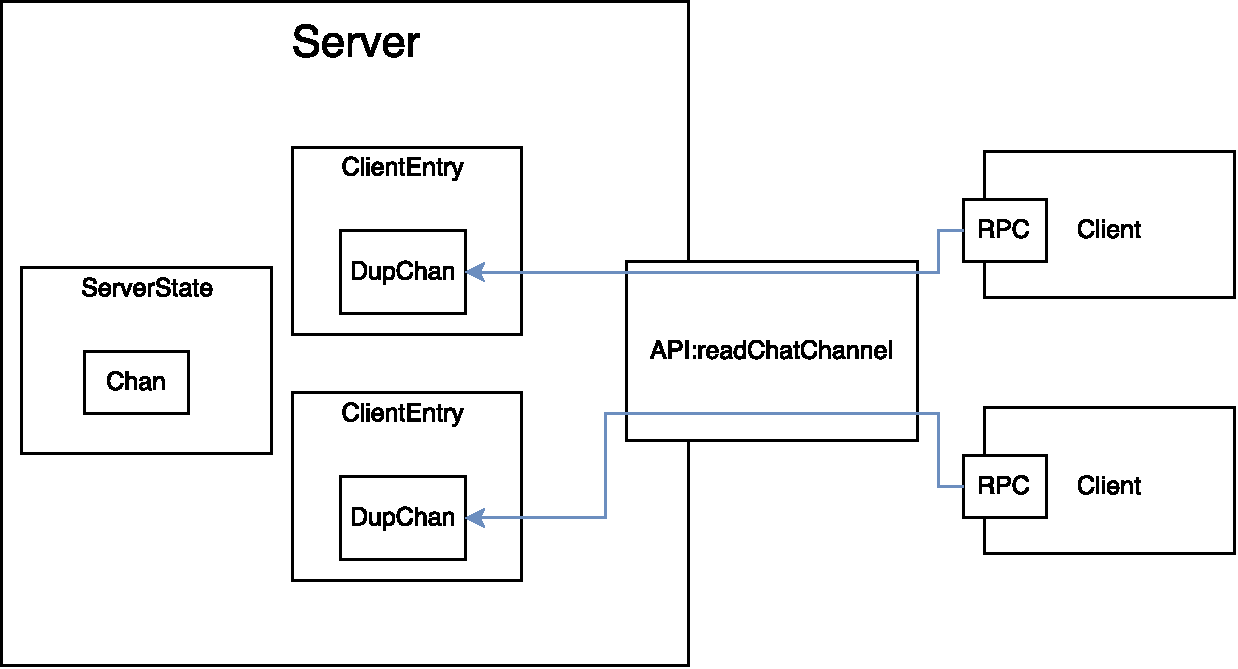
\includegraphics[scale=0.5,width=0.7\textwidth]{figure/readChatFromServer}
    \caption{Visualisation of data flow when a client uses a RPC to remotely access the API function readChatChannel.}
    \label{fig:read-chat-from-server}
\end{figure}

In addition, to properly evaluate the development of a web application using Haste.App it was decided that the lobby should save most of its data in a database, since they are commonly used with web applications. MySQL was chosen as the backend database server and to interface with it from Haskell the libraries \textit{Persistent} \cite{persistent-yesod} and \textit{Esqueleto} \cite{esqueleto-hackage} were used. \textit{Persistent} contains most of the database functionality used in this project, including declaring type-safe SQL tables in Haskell code and Haskell functions that support basic database queries. \textit{Esqueleto} extends the functionality of \textit{Persistent} to allow  custom, type-safe SQL queries that are more complex. At the beginning of the development, all games were stored in a list on the server, but this data was migrated to be stored only in the database to test its properties.

Furthermore, it was decided to test how password management would work with Haste.App, since authentication of users is another important aspect in web development. Therefore, some Haskell libraries offering to hash passwords were considered and it was decided to use \textit{Crypto.PasswordStore} \cite{pwstore-package}. However, since it would take too long to develop a user authentication system, it was decided that users should be able to protect their games with passwords. At first, the passwords were meant to be hashed at the client, but the library was not compatible with Haste. As such the passwords are sent in plain text and hashed at the server.



\subsubsection{Data types of the Lobby}
To create the lobby as previously described, a number of data types were created, which can be seen in \cref{fig:datatypes}. The data types are mostly self-descriptive, but some of the design decisions are illustrated here.

First, two lists were encapsulated in an MVar, namely $ConcurrentClientList$ and $ConcurrentChatList$. They were decided to be MVars since they are passed to the remote server functions at the entry point of the program and then modified inside those functions. This was necessary since it allows them to work in a similar way to a state, and since it allows only one process to access them simultaneously. Originally there was one more MVar list, $ConcurrentGameList$, but it was removed as all game data was instead saved in the database.

Next, there are two $Message$ data types, $ChatMessage$ and $LobbyMessage$. These were created in order to communicate change to clients. They are encapsulated in Concurrent Channels in order to allow the server, via a call from a client, write several messages to a client. These messages are then read via a remote call from a client to the server as illustrated in \cref{fig:reading-channel}.

\begin{figure}[ht!]
    \centering
    \begin{subfigure}{\textwidth}
        \centering
        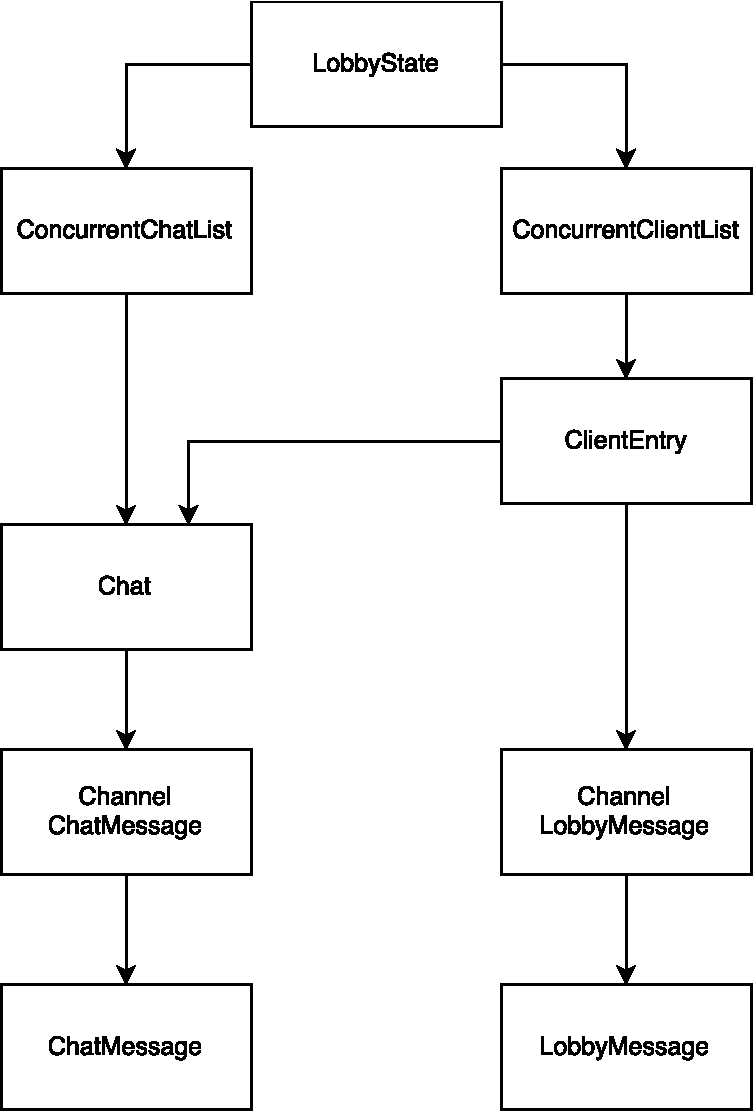
\includegraphics[scale=0.4]{figure/datatypes}
        \subcaption{The diagram displays the hierarchy in which the data types depend on each other.}
    
    \end{subfigure}
    \begin{subfigure}{\textwidth}
        \begin{lstlisting}
type LobbyState = (Server ConcurrentClientList, Server ConcurrentChatList)
type ConcurrentClientList = MVar [ClientEntry]
type ConcurrentChatList = MVar [Chat]

type Chat = (Name, Chan ChatMessage)

type Name = String

data ClientEntry = ClientEntry {sessionID    :: SessionID
                               ,name         :: Name
                               ,chats        :: [Chat]
                               ,lobbyChannel :: Chan LobbyMessage
                               ,gameChannel  :: Chan GameAction}

data ChatMessage = ChatMessage       {from    :: Name
                                     ,content :: String}
                 | ChatJoin
                 | ChatAnnounceJoin  {from :: Name}
                 | ChatLeave
                 | ChatAnnounceLeave {from :: Name}
                 | ChatError         {errorMessage :: String}


data LobbyMessage = NickChange | GameNameChange | KickedFromGame | GameAdded 
                  | ClientJoined| ClientLeft | PlayerJoinedGame | PlayerLeftGame 
                  | StartGame | LobbyError {lobbyErrorMessage :: String}


        \end{lstlisting}
        \subcaption{The data types as they are defined in Haskell. GameAction is defined in the Game section.}
    \end{subfigure}
    \caption{Illustration of the data types in the lobby.}
    \label{fig:datatypes}
\end{figure}


\subsection{Issues encountered with Haste and Haste.App}
\label{sub:issues-during-development}
During the development of the lobby and game a number of issues with Haste and Haste.App arose. The issues were related to working with channels, using the FFI, rendering, dependency management, password management and security, and generating HTML. %Here thgeneratingese issues are described in the context they appeared during the development of the lobby. \todo{Ta bort sista meningen?}

Channels from the $Control.Concurrent$ package does not seem to work with Haste. Writing to a channel works fine, but any other operation such as reading from the channel did not work. The application simply crashes when using any of those functions. 

Using the library function for getting mouse coordinates in a canvas returns the x coordinate relative to the whole screen, and y coordinate relative to the canvas, which of course is not correct. This seems to be a problem with JavaScript and not Haste, since the library function in Haste is implemented using the foreign function interface (FFI), thus calling JavaScript code.

Moreover, the highlighted bitmaps in the game are not always rendered on the canvas, and it seems to be arbitrary when the rendering starts. It is assumed that the issue related to rendering the highlighted bitmaps is caused by a bug in the Haste compiler.


In addition, problems with dependencies with GHC and Haste also exists and are discussed in more detail in \cref{sub:dependencies}. Such a problem was encountered when using the \textit{Data.UUID} library for giving games a unique identifier. The library cannot be installed with Haste, thus forcing a very sharp separation between Server and Client code. 

Furthermore, as described in \cref{sub:lobby-development} passwords are sent in clear text to the server to be hashed. Sending the passwords in clear text revealed an important issue with Haste.App: Haste.App does not provide secure web sockets. Even when forcing an HTTPS connection via the web server the web sockets used by Haste always default to insecure. 


Generating HTML using Haste was a tedious task. The functions that operate on HTML elements, such as $<div>$ and $<body>$, work by first getting an element using its \textit{id} and then modifying that element. It works in the same way as generating an entire HTML page from JavaScript would. The difference between writing a simple HTML tree in Haste compared to pure HTML can be seen in \cref{fig:HTML-generation}. There are a couple of libraries developed for Haste that attempt to simplify generating HTML. Most of these libraries are, however, not up to date and will not work with the current version of Haste due to the rapid development of Haste itself. 

\begin{figure}[H]
    \centering
\begin{subfigure}[b]{\textwidth}
\begin{lstlisting}
parentDiv <- newElem "div" `with`
    [
        attr "id"    =: "parent-div",
        attr "class" =: "input-group"
    ]

inputField <- newElem "input" `with`
    [
      attr "type"  =: "text",
      attr "id"    =: "text-field",
      attr "class" =: "form-control"
    ]

buttonSpan <- newElem "span" `with`
    [
      attr "class" =: "input-group-btn"
    ]
button <- newElem "button" `with`
    [
      attr "id"    =: "input-button",
      attr "type"  =: "button",
      attr "class" =: "btn"
    ]
buttonText <- newTextElem "Change"

appendChild button buttonText
appendChild buttonSpan button
appendChild parentDiv inputField
appendChild parentDiv buttonSpan
appendChild documentBody parentDiv

\end{lstlisting}
\caption{Creating HTML in Haste}
\end{subfigure}


\begin{subfigure}[b]{\textwidth}
\begin{lstlisting}[language=HTML]
<body>
    <div id="parent-div" class="input-group">
        <input type="text" id="text-field" class="form-control">
        <span class="input-group-btn">
            <button id="input-button" type="button" class="btn">
                "Change"
            <button>
        </span>
    </div>
</body>

\end{lstlisting}
\caption{The same HTML in an .html file}
\end{subfigure}

\caption{Comparison of generating HTML in pure .html files and in Haste}
\label{fig:HTML-generation}
\end{figure}

However, an alternative to writing the HTML in Haste would be to have several HTML files that could be switched to during the use of the lobby. However, this exposed an issue with Haste.App: When the HTML file was switched the client disconnects from the server and then reconnects. Since the client has to reconnect, the server cannot easily identify this client as being the same as before. While this is an issue that can be bypassed by adding some identification to the client stored in HTML5 Local Storage (that Haste has support for), it was considered out of the scope of the project.

\newpage
\section{Results}
The aim of this project was to evaluate, based on a few topics, how suitable Haste.App is for web development. The topics were: Performance, stability and programmer productivity. The results are split into two parts. The first part addresses what was created, namely the game and the lobby and their respective functionality. The second part presents the results of the three points of interest and is evaluated as described in \cref{sec:method}.

\subsection{Game and Lobby implementation results}
\label{sub:game-lobby-results}
The game of Chinese Chequers was implemented according to description in \cref{sec:game-rules}. The resulting graphics can be seen in \cref{fig:gameGraphics}.


The implementation of the lobby system resulted in a system that does the following things:
\begin{itemize}[noitemsep]
    \item Start a game that others can join.
    \item Changing settings of a game, including name, password and, max number of players allowed.
    \item Chat with other players.
    \item Saving games and players in an external database.\\
\end{itemize}


The source code is available on GitHub, allowing a deeper review of the implementation:
\begin{itemize}[noitemsep]
    \item Game: \url{https://github.com/DATx02-16-14/ChineseCheckers}
    \item Lobby: \url{https://github.com/DATx02-16-14/Hastings}
    %\item Performance test scripts: \url{https://github.com/DATx02-16-14/scripts}
\end{itemize}



\subsection{Results regarding performance}
\label{sub:performance-results}
The performance of the application is measured by, as stated in \cref{sub:method-performance}, the bandwidth required and system resources used. The bandwidth considered is primarily the data required to send the JavaScript since the data required to send images, text, and other static content is not unique to Haste.App. Moreover, the bandwidth needed when communicating with the server during use is also considered to make sure the client-centric programming model does not yield an unnecessary amount of network traffic. Furthermore, the system resources used on the server is measured, in respect to how many players are online. In addition, the system resources used on the client is measured.


\subsubsection{Server-Side performance}
\label{subsub:server-performance-results}
Using \textit{watir} it was possible to simulate 80 clients which joined the lobby, wrote messages in the chat and created games. The 80 clients were split up on four computers with 20 simulated clients each. The CPU usage, memory usage, load average and network traffic can be seen in \cref{fig:cpu-results} and \cref{fig:cpu-results-attachment}, \cref{fig:memory-results} and \cref{fig:memory-results-attachment}, \cref{fig:network-results} and \cref{fig:network-results-attachment}, \cref{fig:load-average-results} and \cref{fig:load-average-results-attachment}, respectively. The server running the application has 8 GB RAM and an Intel(R) Core(TM)2 Duo CPU E8400 3.00GHz, running Ubuntu 15.10. The full system specifications can be found in \cref{sub:system-specs}. Two tests were performed and are described below along with observations on CPU, memory, network traffic, and load average.

The first test showed the load when creating games on the server and as such tested performance when accessing the database. At 14:30 the 80 clients joined a game. At 14:45 the 80 clients created games and upon creating the games they change the games name, password and max amount of players. At 15:05 all clients start to leave the server.

The second test evaluated pure Haste.App performance by chatting in the server, it did not require any access to the database. The 80 clients joined at 16:25, and at 16:40 they start to chat. At 16:50 the clients then disconnect from the server.

Firstly, regarding CPU on the server, which is illustrated in \cref{fig:cpu-results} and \cref{fig:cpu-results-attachment}, it increases to about 5\% when 80 clients join the server. It can be seen that the most CPU intensive tasks occur when games are created and settings on them changed. This is either because of passwords for the games are set and then hashed on the server or because all game data is entered into the database and as such when a setting is changed and a game created the database is accessed. When chatting, that is only sending messages through Haste.App, the CPU usage stays at roughly 5\%.
\begin{figure}[ht!]
\centering
    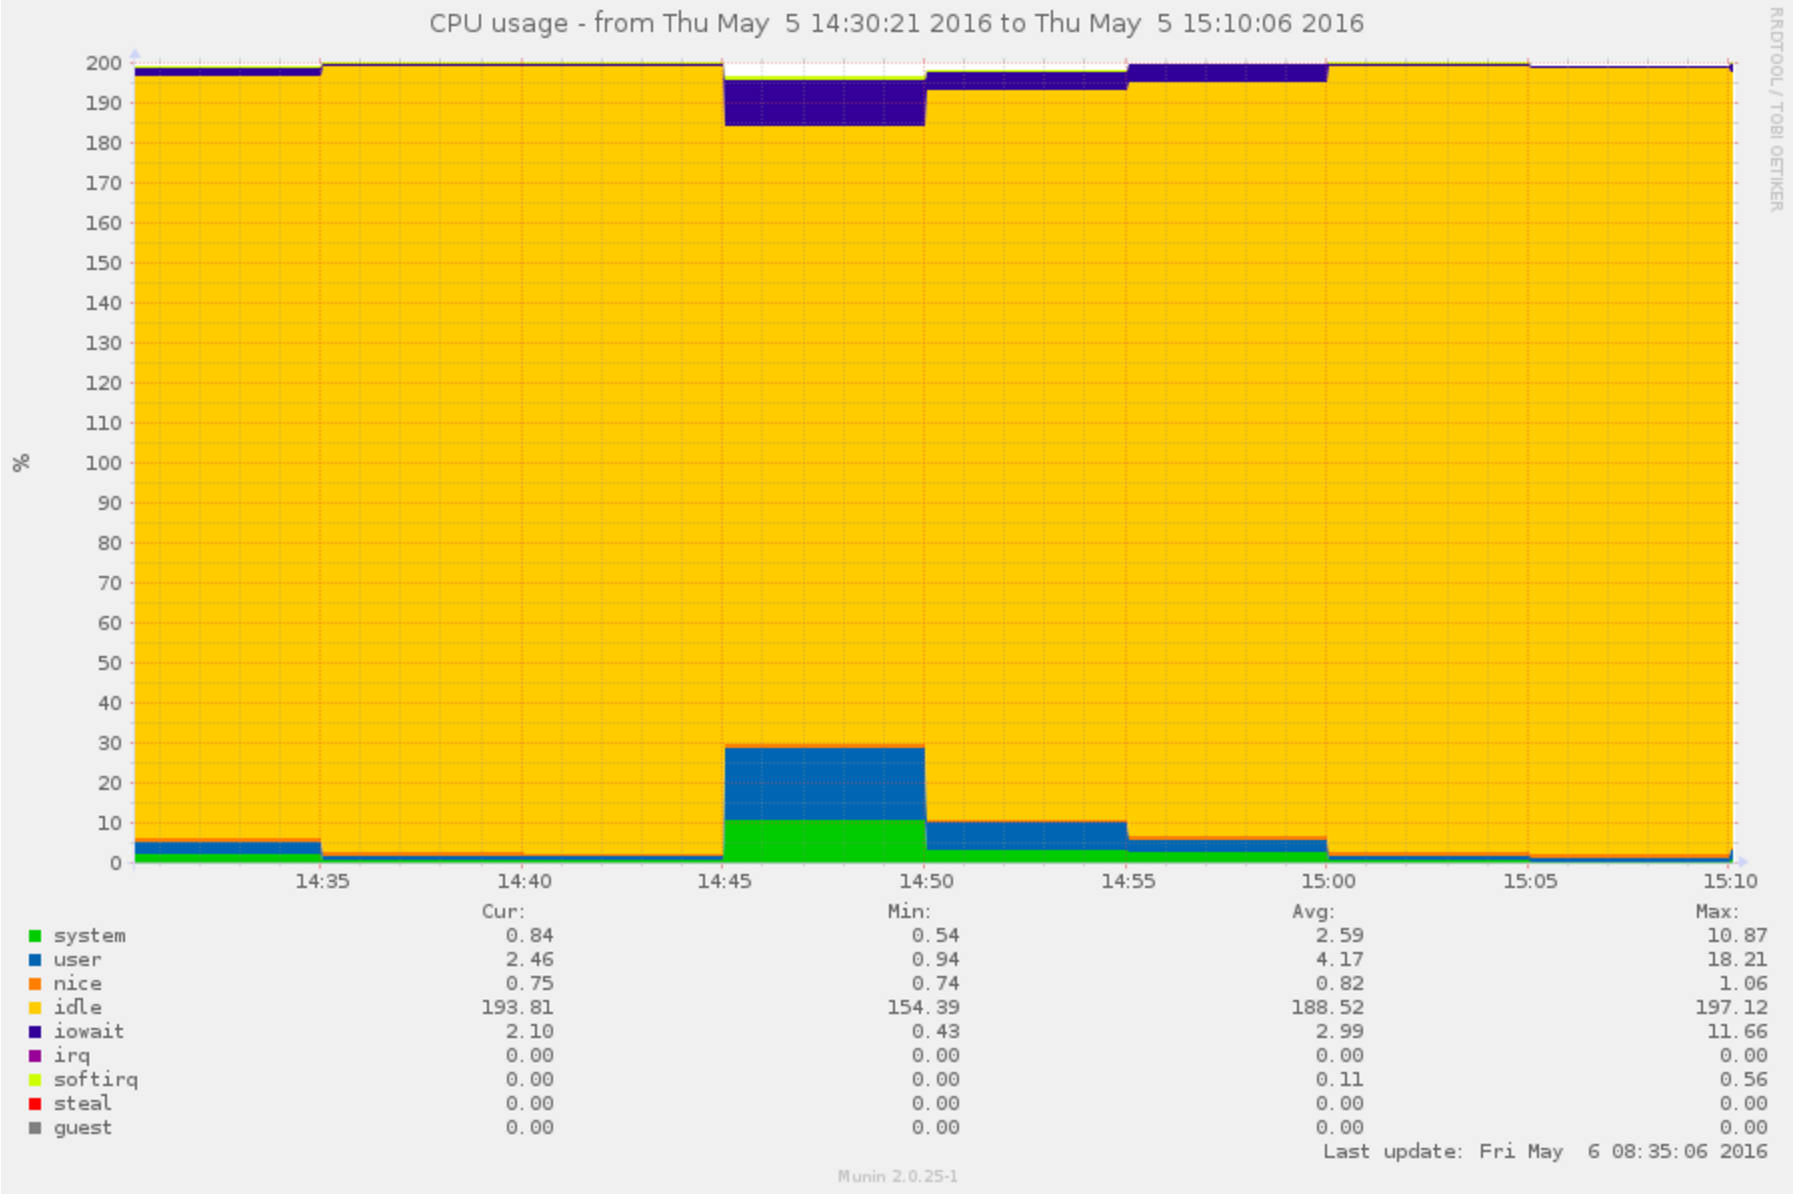
\includegraphics[width=0.9\textwidth]{figure/serversidePerformance/2016-05-05-game-test-cpu2.png}
    \caption{CPU usage on the server during the first test}
    %\caption{CPU usage on the server during the two tests}
    \label{fig:cpu-results}
\end{figure}

The memory usage on the server, which is illustrated in \cref{fig:memory-results} and \cref{fig:memory-results-attachment}, stays about the same during both tests. The only time where there is noticeable memory usage is when the initial connection is established. 

\begin{figure}[ht!]
\centering
    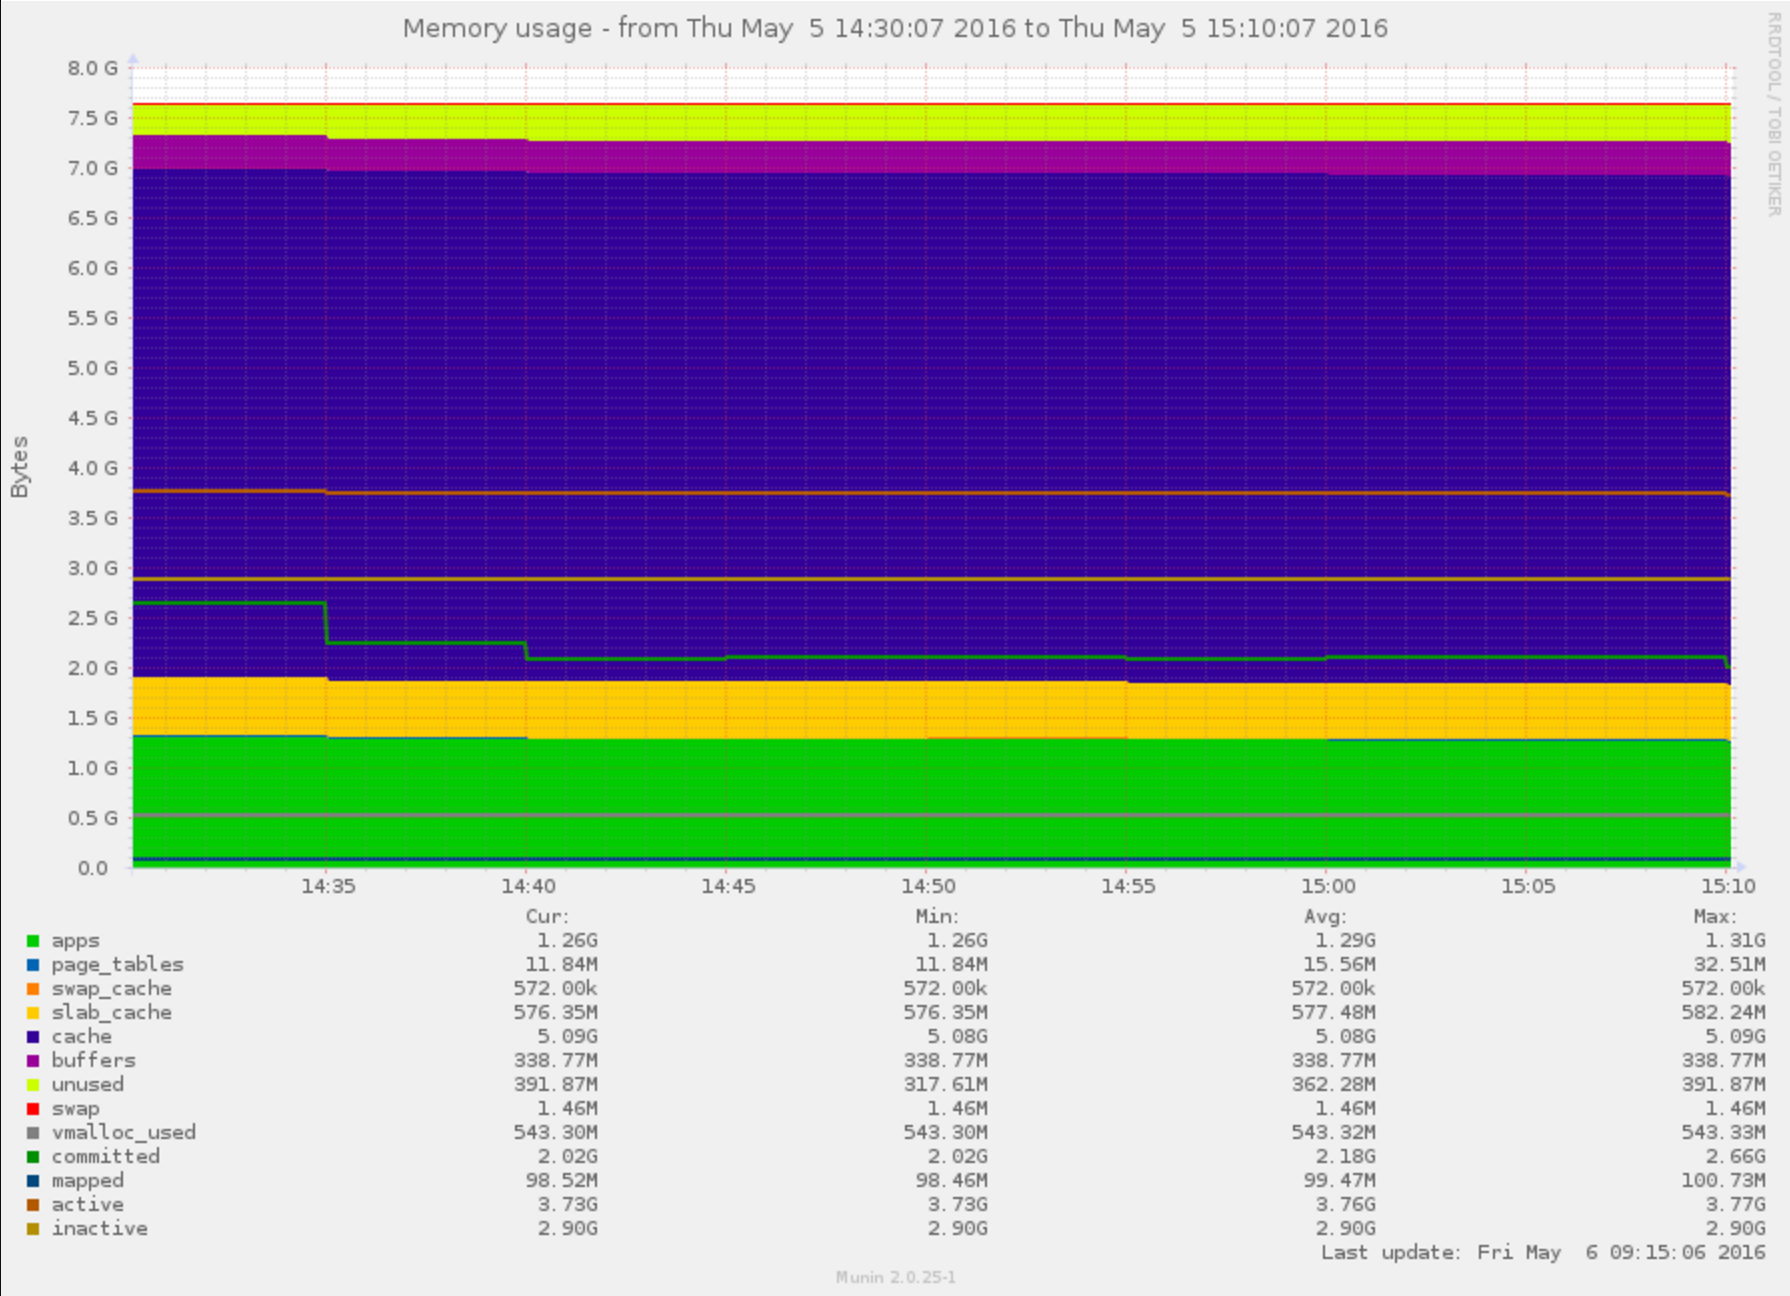
\includegraphics[width=0.9\textwidth]{figure/serversidePerformance/2016-05-05-game-memory.png}
    \caption{Memory usage on the server during the first test}
    %\caption{Memory usage on the server during the two tests}
    %\caption{Server performance when 80 clients joined the server(14:25), created games and changed their settings(14:45-15:00) and then left(15:10)}
    \label{fig:memory-results}
\end{figure}

Furthermore, network traffic on the server during the two tests are shown in \cref{fig:network-results} and \cref{fig:network-results-attachment}. The server sends more data than it receives when the clients connect. During the phase where the clients either chat or create games, the server sends about the same amount of data as it receives as all clients receive messages as described in \cref{sub:lobby-development}. When disconnecting some data is sent, but not much.

\begin{figure}[H]
\centering
    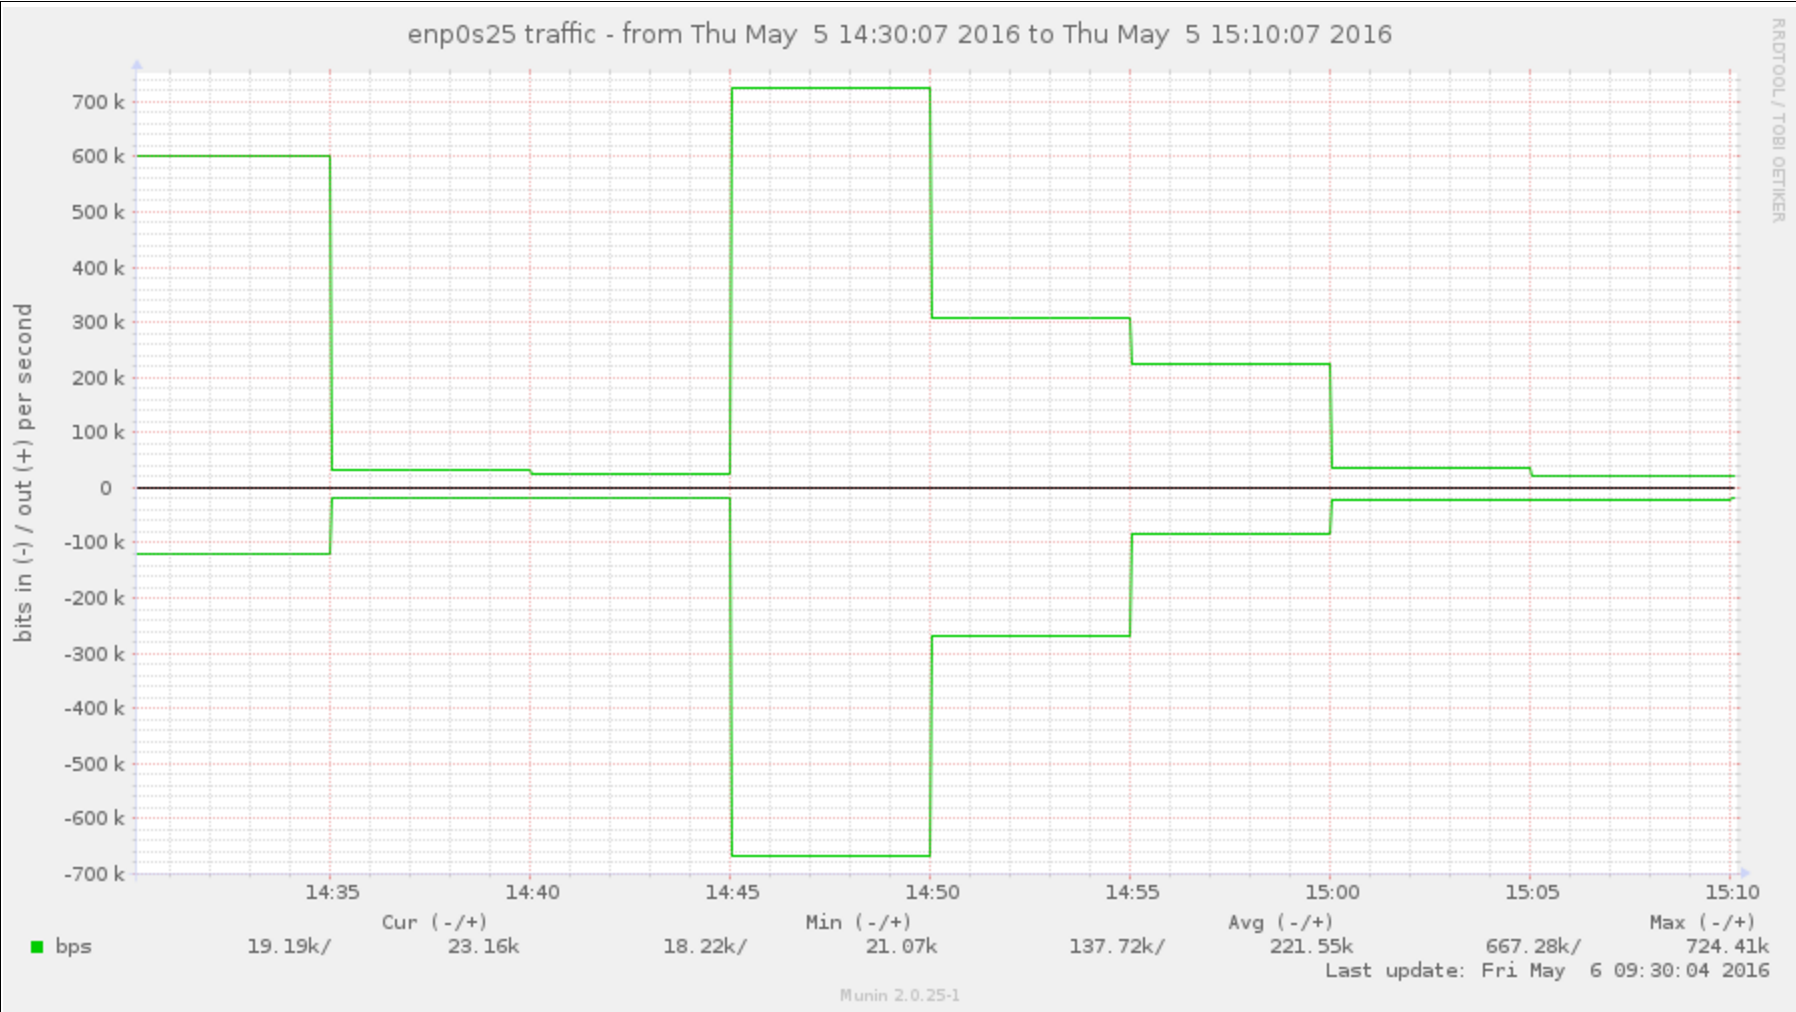
\includegraphics[width=0.9\textwidth]{figure/serversidePerformance/2016-05-05-network-traffic-game.png}
    \caption{Network traffic on the server during the first test}
    
    %\caption{Network traffic on the server during the two tests}
    %\caption{Server performance when 80 clients joined the server(14:25), created games and changed their settings(14:45-15:00) and then left(15:10)}
    \label{fig:network-results}
\end{figure}

The load average can be seen in \cref{fig:load-average-results} and \cref{fig:load-average-results-attachment}. The load stays below one throughout the tests which indicates that no process has to wait to be run. The max load average is 0.43, which is not especially high since 1.0 indicates that one process is waiting for CPU time.

\begin{figure}[H]
    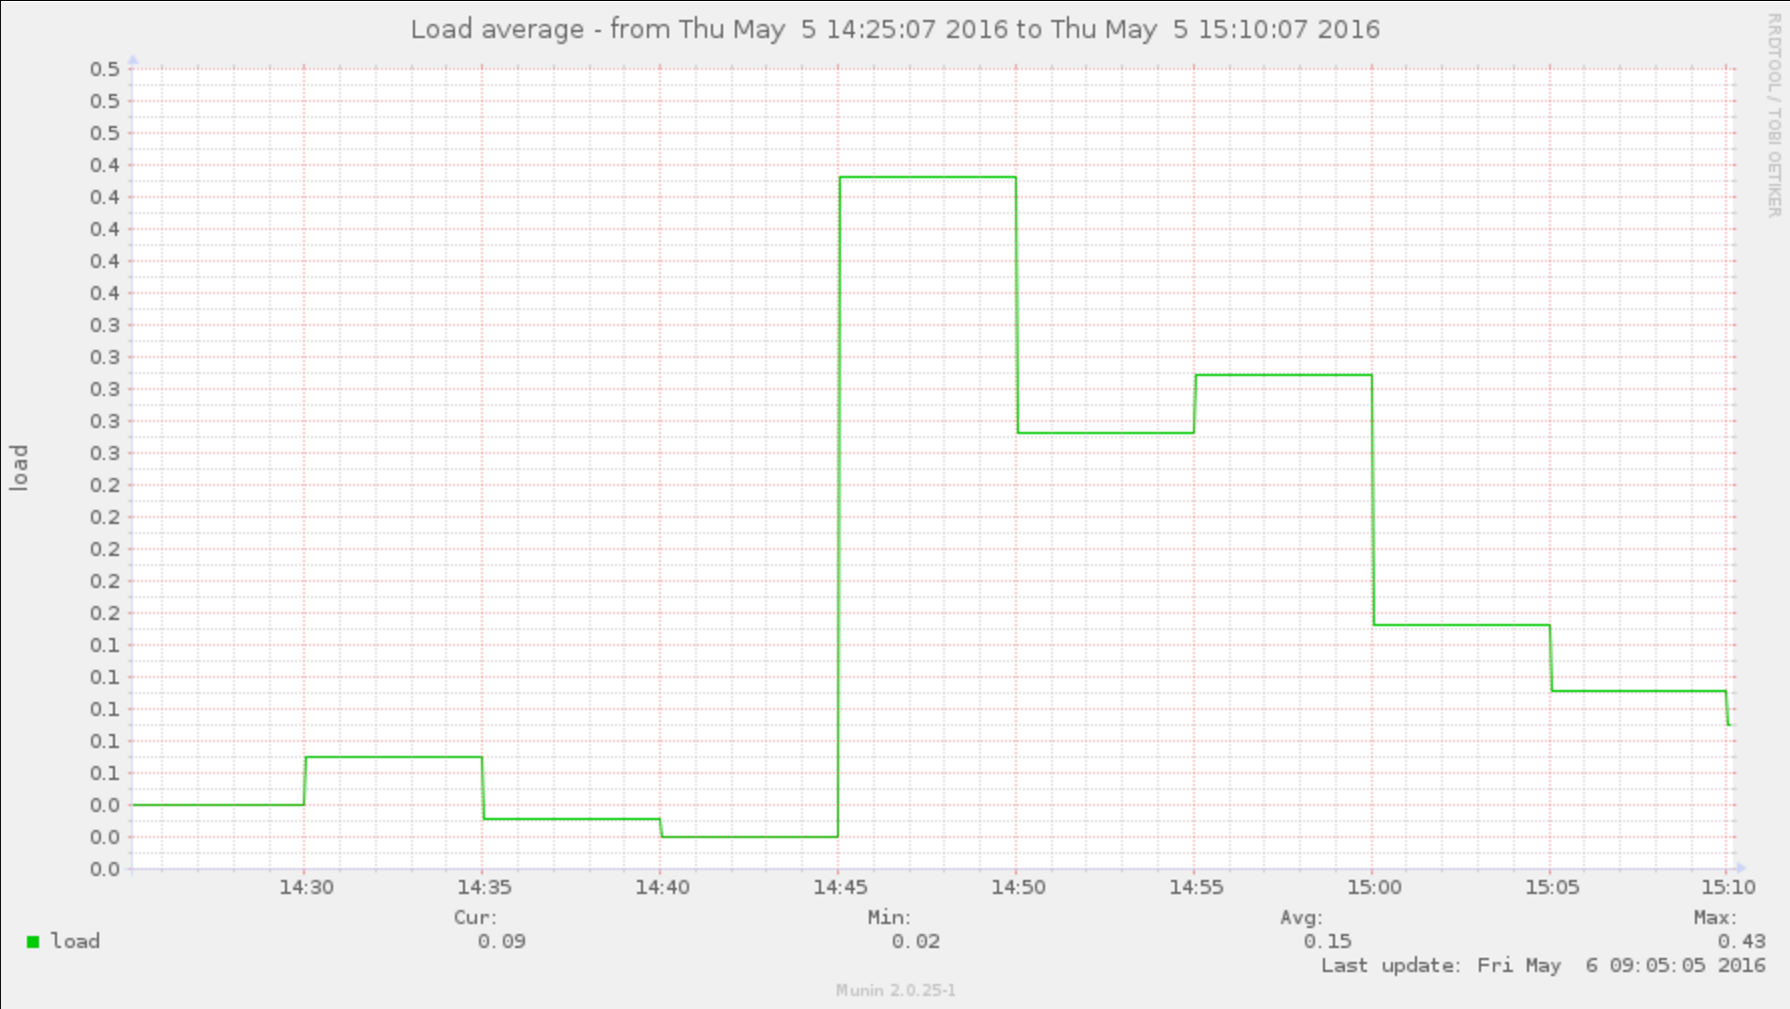
\includegraphics[width=0.9\textwidth]{figure/serversidePerformance/2016-05-05-load-average-game-test.png}
    \caption{Load average on the server during the first test}
    %\caption{Server performance when 80 clients joined the server(14:25), created games and changed their settings(14:45-15:00) and then left(15:10)}
    \label{fig:load-average-results}
\end{figure}


\subsubsection{Client-Side performance}
\label{subsub:client-performance-results}
The measured performance on the client-side was done in two parts. The JavaScript was profiled three times, with 0, 30 and 90 games created in the lobby respectively, results from that profiling are shown in \cref{fig:hastings-performance}. The figure shows that the relationship between the number of games created in the lobby and the total loading time for the website has a linear relationship. Additionally, in \cref{fig:hastings-comparison} two other websites that offer a lobby system were profiled, \textit{brasee.com} and \textit{lichess.org}. Lichess is a very popular website with 6000 concurrent users and 1500 simultaneous games at the time of profiling. Brasee, on the other hand, is not as popular with only a couple of games and about as many users online when the profiling was run. Nonetheless, it is interesting to note that while Lichess was noticeably slower, it also had a lot more games and players connected.

\begin{figure}[H]
    \centering
    \begin{subfigure}{0.32\textwidth}
        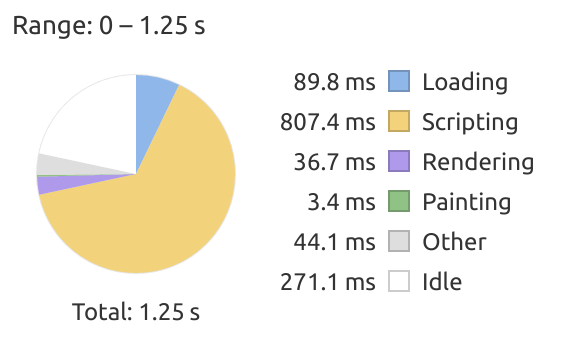
\includegraphics[width=\textwidth]{figure/clientsidePerformance/graph1.png}
        \subcaption{1 player connected and 0 games created.}
    \end{subfigure}
    \begin{subfigure}{0.32\textwidth}
        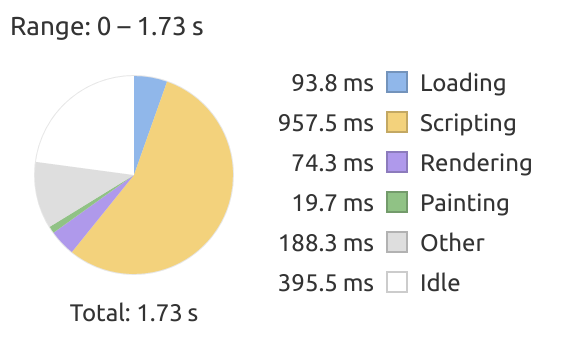
\includegraphics[width=\textwidth]{figure/clientsidePerformance/graph30games1.png}
        \subcaption{1 player connected and 30 games created.}
    \end{subfigure}
    \begin{subfigure}{0.32\textwidth}
        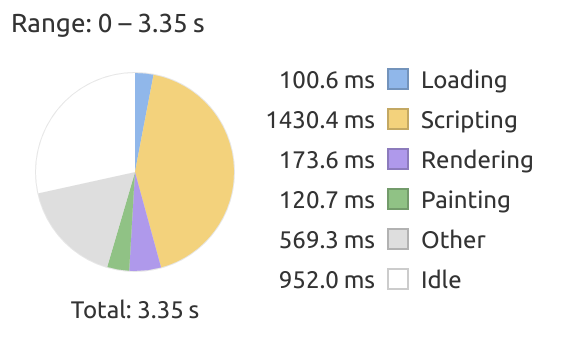
\includegraphics[width=\textwidth]{figure/clientsidePerformance/graph90games1.png}
        \subcaption{1 player connected and 90 games created.}
    \end{subfigure}
    
    \caption{Breakdown of computation time when loading the website in Chrome.}
    \label{fig:hastings-performance}
\end{figure}


\begin{figure}[H]
    \centering
    \begin{subfigure}{0.32\textwidth}
        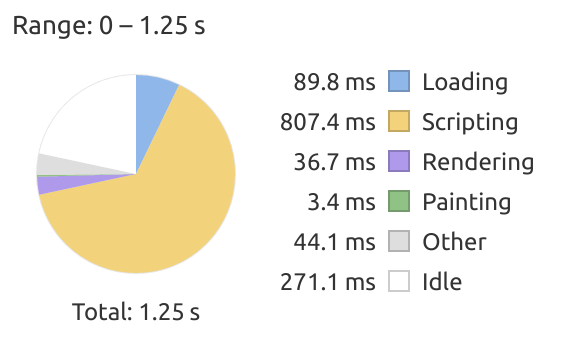
\includegraphics[width=\textwidth]{figure/clientsidePerformance/graph1.png}
        \subcaption{Loading our website with 0 games created.}
    \end{subfigure}
    \begin{subfigure}{0.32\textwidth}
        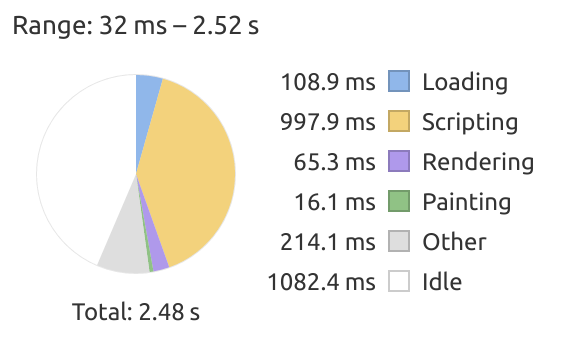
\includegraphics[width=\textwidth]{figure/clientsidePerformance/braseegraph1.png}
        \subcaption{Loading of the lobby on Brasee.}
    \end{subfigure}
    \begin{subfigure}{0.32\textwidth}
        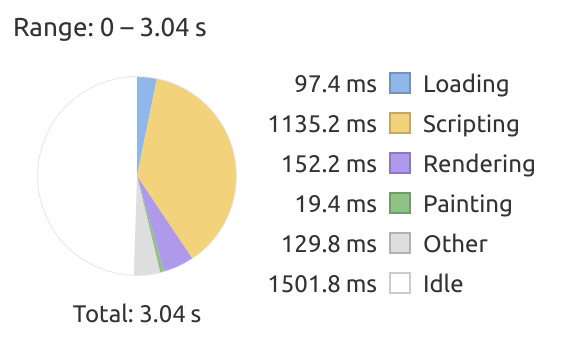
\includegraphics[width=\textwidth]{figure/clientsidePerformance/ligraph1.png}
        \subcaption{Loading of the lobby on Lichess.}
    \end{subfigure}
    
    \caption{Breakdown of computation time when loading three similar websites in Chrome.}
    \label{fig:hastings-comparison}
\end{figure}

\subsubsection{Bandwidth when using Haste.App}
In order to profile the bandwidth used by the websites, the program \textit{Wireshark} was used. All packets sent and received by the host address during a period of ten minutes were captured and analysed. In \cref{tab:site-comparisons}, data is differentiated by static and dynamic data. Static data is images and website content that are sent on page load. Dynamic data is data transmitted in response to an event by the application, for example, a player joining the lobby or when a chat message is sent. 

In \cref{tab:site-comparisons} there are a couple of noteworthy differences. Firstly, Brasee has considerably more static data which can be attributed to the large number of images on that website compared to the others. Secondly, the Lichess lobby sent more dynamic data; probably because Lichess had a greater number of players connected.

\begin{table}[H]
\centering
\begin{tabular}{|l|l|l|l|}
\hline
\textbf{Web Site} & \textbf{Total Data Sent}(kb) & \textbf{Dynamic data}(kb)     & \textbf{Static Data}(kb)\\ \hline
Lichess Lobby  & 1185,737         & 1181,276    & 4,461       \\ \hline
Lichess Game   & 122,067          & 116,512     & 5,555       \\ \hline
Brasee Lobby   & 1496,903         & 254,435     & 1242,468    \\ \hline
Brasee Game    & 2108,192         & 692,241     & 1415,951    \\ \hline
Our Lobby      & 281,692          & 278,035     & 3,657       \\ \hline
Our Game       & 162,067          & 156,705     & 5,362       \\ \hline
\end{tabular}
\caption{Data sent (in kilobytes) between the client and server for different lobby and game systems during 10 minutes.}
\label{tab:site-comparisons}
\end{table}

\subsection{Results regarding stability}
\label{sub:stability-results}
The stability of the application was considered out of four aspects, as defined in \cref{sub:method-stability}: updating the server, a client connecting with outdated JavaScript, runtime errors on the Server, and runtime errors on the client. 

Because of the static type checking if Haskell the amount of runtime errors related to types on the client were reduced compared to writing JavaScript code. They are reduced since the static type checking captures all type errors in compile time. It did, however, not completely rid the application from them. Moreover, there are errors that are recoverable which seem to be inherent to Haste, namely when there is an HTML input field. The first character written into the field throws an error with the message:
\begin{align*}
    \textit{Uncaught [object Object]}
\end{align*} 
When continuing to write it throws an error with the message for every letter typed:
\begin{align*}
    \textit{Uncaught Infinite loop!}
\end{align*}
These errors, however, do not seem to have any effect on the application.

The unrecoverable errors that can occur do so when working with the DOM, and specifically when trying to retrieve objects with an \textit{ID} that does not exist. This is, however, a problem that has to be dealt with both when using Haste and when using JavaScript.

Moreover, the server also very rarely has runtime errors. The programming model of Haste.App, with type safe network communication, appears to work very well. There has been no instance of a crash or bug occurring because of a network communication problem.

Updating the server, however, seems to be a prominent issue with Haste.App. There is currently no way of updating the server without disconnecting all clients connected. As the communication is handled via HTML5 WebSockets, these close when the server is restarted and there is no way in Haste.App to resume the same connection. The client has to reset the connection and thus it has to restart from the same state it was in when it first connected to the server. There is no way to keep current connections alive while updating the server so that new connections receives the updated state.

Since the code is compiled twice, the server and the client code needs to match. Matching the code can be tedious since the HTML has to be placed/updated at the web servers root and then the server has to be restarted. Should one of the two steps not be performed, the application can enter a faulty state and crash.

Moreover, to ensure the logical correctness of the code, the testing library \textit{QuickCheck} was used. The ability to use a powerful testing library helps in eliminating logical errors in the code. As such, \textit{QuickCheck} has helped to ensure the stability of the application.

Furthermore, there is no memory leakage on the server. The server application was left running for seven days during which the application was moderately used. During this time there were no evident increase in memory usage on the server.

\subsection{Results regarding programmer productivity}
\label{sub:programmer-productivity-results}
Programmer productivity when writing a web application using Haste.App was heavily influenced by a number of factors. A large influence is that all code is written in Haskell, compared to writing JavaScript client-side and some language server-side. Other influences on programmer productivity have been debugging and runtime errors, database usage, the linear, client-centric approach taken by Haste.App, and the fact that the whole application is written in the same language and the same project. The lines of code in the complete application are also compared to other similar applications and games.

\subsubsection{Haskell versus JavaScript during development}
\label{subsub:haskell-vs-js-during-development}
An advantage to writing the client-side code using Haskell instead of JavaScript has been the static type system of Haskell. Instead of manually checking the types of a function or data type (or object in JavaScript), one can rely on the static type checking to report any type errors. Allowing types to be checked during compilation has reduced the number of bugs encountered to a very limited set of runtime errors. In addition, since the type checking can also be used over the network, type checking network code is an easy matter.

Another advantage of Haskell is the clear separation between pure code and code with side effects. Most of the code with side effects in the developed game were Haste code. The graphical and network implementations are the parts where Haste was needed, while the game logic was written purely in Haskell. This clean separation made it easy to use \textit{QuickCheck} to test the pure and impure code as shown in \cref{fig:quickchecking}, and \cref{fig:quickcheck-monadic}.

\begin{figure}[ht!]
    \begin{lstlisting}
-- |Property that checks that a square is not empty after having piece put into it.
prop_putPiece :: TableCoords -> OnlyPiece -> Bool
prop_putPiece (TableCoords (t, _, coord)) (OnlyPiece p) =
    squareContent (putPiece t p coord) coord /= Empty
    \end{lstlisting}
    \caption{Testing pure code using QuickCheck.}
    \label{fig:quickchecking}
\end{figure}    

\begin{figure}[ht!]
    \begin{lstlisting}
-- |Property that makes sure a game can be properly created.
prop_createGame :: [ClientEntry] -> Int -> Property
prop_createGame clientList maxPlayers = monadicIO $ do
  pre $
    not (null clientList) &&
    maxPlayers /= 0

  let sid = sessionID $ head clientList
  let playerName = name $ head clientList
  run preProp

  --Setup test preconditions.
  clientMVar <- run $ newMVar clientList

  run $ PlayerDB.saveOnlinePlayer playerName sid
  uuid <- run $ Server.Game.createGame clientMVar sid maxPlayers

  game <- run $ GameDB.retrieveGameBySid sid

  --Cleanup test
  run postProp

  assert $
    --Check that the UUID returned exists.
    isJust uuid &&
    --Check that the game exists in the database.
    isJust game &&
    --Check that the max amount of players is correct.
    (Fields.gameMaxAmountOfPlayers . Esql.entityVal . fromJust) game == maxPlayers
    \end{lstlisting}
    \caption{Testing impure code in the IO monad using QuickCheck.}
    \label{fig:quickcheck-monadic}
\end{figure}

However, when writing a client-server application in Haste.App almost all client and server specific code has side effects. The client code is naturally placed in the \textit{Client} monad, and the server code in the \textit{Server} monad. The client mostly creates and updates HTML, which is naturally side-effecting. Furthermore, the server code mostly modifies a state, either in a database or a synchronous variable, both of which are also side-effecting. However, most code is easily testable by lifting the functions into the IO monad, which \textit{QuickCheck} supports natively.


\subsubsection{Runtime errors and debugging}
\label{subsub:runtime-errors-debugging}
One disadvantage of using Haste.App is that when runtime errors occur in the JavaScript code they can be hard to debug properly. This is because the JavaScript generated by Haste is hard to read by humans, even if the debug flag is supplied to skip some of the optimisation and minimisation steps. Also, as mentioned in \cref{sub:stability-results}, the error messages that are generated by JavaScript does not indicate what caused the error or which Haskell function gave the error. 

Furthermore, it is problematic to use a debugger on the generated JavaScript. A debugger enables the programmer to pause the execution of a program at a particular point and look at the current state of the program. While it is possible to use a debugger on the code, the code is still very cryptic in its construction. Because debugging is difficult, it can be hard to find where the faulty computations occur.


\subsubsection{Database usage influence on programmer productivity}
\label{subsub:database-results}
There are several benefits to programmer productivity when working with a database library that extends Haskell's type system to the SQL domain. The most notable positive aspects include declaring native Haskell types as database tables and the fact that virtually all SQL errors are detected at compile time. However, one disadvantage is that the syntax is different to traditional SQL syntax.

The advantages manifest primarily in two distinct cases. Firstly, when writing functions that interface with the database there is no need to convert between types that the database can understand and types that Haskell can understand. Secondly, when a change is made to the structure of a database table, the error is detected at compile time. When using ordinary SQL such errors are not detected. Instead, the error occurs when the application is running. If the code that causes the error is not executed very often it can take a long time before the error is detected. 

A disadvantage, however, is the difference in syntax between SQL and the syntax employed by the library \textit{Esquelto}, which is illustrated in \cref{fig:esqueleto-vs-sql}. The figure shows an SQL query that retrieves all players that are currently in a game, along with the Haskell code that generates an equivalent query. A notable difference is the fact that the Haskell code is more verbose than the SQL code, and the Haskell code uses operators that are not immediately obvious what they do. Because the library uses such a different syntax, it could affect programmer productivity since a programmer that is already accustomed to SQL has to learn how to use \textit{Esqueleto} as well.



\begin{figure}[ht!]
\begin{subfigure}[]{\textwidth}
\begin{lstlisting}[language=SQL]
DELETE FROM PlayersInGame
  WHERE game = 'gameKey' AND player = 'playerSessionId';
\end{lstlisting}
\subcaption{SQL statement that removes a specific player from a specific game.}
\end{subfigure}

\begin{subfigure}[]{\textwidth}
\begin{lstlisting}[language=Haskell]
removePlayerFromGame sessionID gameKey = runDB $
  delete $ from $ \playersInGame ->
    where_ (playersInGame ^. PlayerInGameGame ==. val gameKey
        &&. playersInGame ^. PlayerInGamePlayer ==. val sessionID)
\end{lstlisting}
\subcaption{Esqueleto code that generates the SQL statement in (a)}
\end{subfigure}

\caption{The difference between Esqueleto syntax and SQL syntax.}
\label{fig:esqueleto-vs-sql}
\end{figure}


\subsubsection{A client-centric, seamless, and linear program flow}
The seamless, linear, client-centric approach of Haste.App has boosted programmer productivity. Not only the fact that the programmer is relieved of dealing with the network communication, and as such allow the type-checking to check remote calls. It is also helpful that the entire application is written in the same language and driven by the client. However, the fact that the same sources are compiled twice with different compilers has led to some issues with dependencies.

Firstly, the fact that the programmer never has to consider the network communication may not be a large problem if one is comfortable with network communication. For someone new to the field it can be a huge relief. As such it has a positive effect on programmer productivity since the communication is built into Haste.App. The fact that all network communication is type checked also has positive effects on programmer productivity since it removes confusing network errors from the application.

Using the same programming language throughout the application also has a positive effect on programmer productivity. Both because a programmer does not have to be confident in two different languages and because the same code can be reused on both the client and on the server. However, during this project barely any of the code written has appropriate reuse on both the client and the server side. Therefore, the effects of reusability might be rather small. It is however still useful not having to change language when switching between client code and server code.

Moreover, the same sources are compiled twice, but all libraries that work with GHC does not work with Haste, which is a problem. Since all libraries do not function with both compilers, a separation had to be made between the code that is compiled with GHC and Haste respectively. The separation took some time to do, and it made some code confusing.

The client-centric approach of Haste.App has helped reduce the amount of errors that can occur because the client and server do not execute code in parallel. Because the client is the driving force, it is easier to reason about the state of the program since the server will not execute any code without the client explicitly telling it to. Furthermore, there is no need to handle the client waiting for information from the server; the client calls a blocking function that requests data from the server.


\subsubsection{Project standards and module structure}
Neither Haste nor Haste.App brought any project structure standards, which may result in the need to refactor code after some development, which can be unproductive. In the game and lobby there was a lack of structure in multiple areas: how to create and update views, extracting pure logic to enable testability and also separating client and server code. The resulting project structure can be seen in \cref{fig:module-dependencies}.

\begin{figure}[ht]
    \centering
    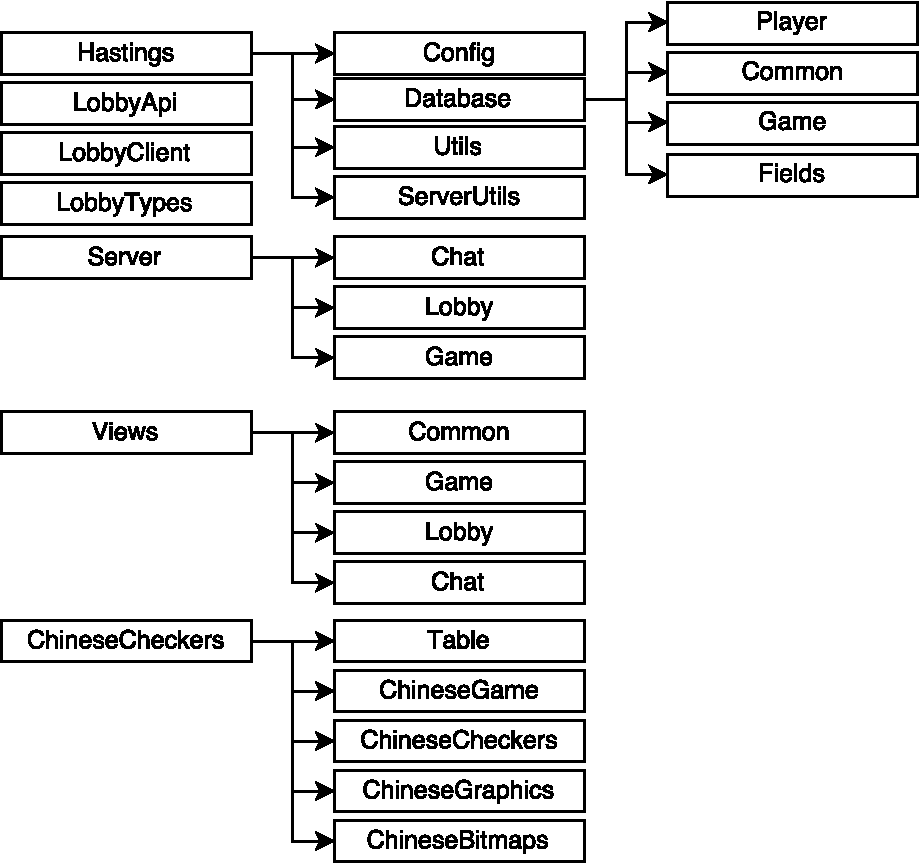
\includegraphics[scale=0.3,width=0.5\textwidth]{figure/module-dependencies}
    \caption{The resulting module structure in the project.}
    \label{fig:module-dependencies}
\end{figure}


\subsubsection{Lines of code}
\label{subsub:lines-of-code-results}
The source lines of code (SLOC) in the finished game and lobby were compared to other similar applications, both games and lobby systems in the \cref{tab:sloc-comparison}. The applications that were compared to can be found at GitHub:
\begin{enumerate}
    \item Offline two-player Chinese Chequers in C++ called Checkers, here referred to as Chinese Chequers \#1, \url{https://github.com/chandramaloo/Checkers}
    \item Offline full Chinese Chequers in Java called Chinese\_Checkers, here referred to as Chinese Chequers \#2, \url{https://github.com/rycnhoj/Chinese_Checkers}
    \item Offline two-player Chinese Chequers with an additional puzzle mode in Java called chinese-checkers, here referred to as Chinese Chequers \#3, \url{https://github.com/mavlee/chinese-checkers}
    \item Web application for Chinese Chequers with backend in Java called ChineseCheckersWebApp, \url{https://github.com/liornaar/ChineseCheckersWebApp}
\end{enumerate}

\begin{table}[H]
    \centering
    \begin{tabular}{|l|l|}
        \hline
        \textbf{Name}  & \textbf{SLOC}                                      \\ \hline 
        \multicolumn{2}{|c|}{\textit{This project's applications}}          \\
        This project's Chinese chequers     & 633 Haskell                   \\ \hline
        This project's lobby system         & 1754 Haskell                  \\ \hline
        Lobby integrated with game          & 2387 Haskell                  \\ \hline 
        \multicolumn{2}{|c|}{\textit{Other applications}}                   \\
        Chinese Chequers \#1                & 483  C++                      \\ \hline
        Chinese Chequers \#2                & 1011 Java                     \\ \hline
        Chinese Chequers \#3                & 1377 Java                     \\ \hline
        ChineseCheckersWebApp               & 2404 Java, 1277 JavaScript    \\ \hline 
        
    \end{tabular}
    \caption{SLOC comparison between the developed application and other similar applications.}
    \label{tab:sloc-comparison}
\end{table}

The results in \cref{tab:sloc-comparison} illustrate that an application written in Haskell and Haste.App is smaller in all cases but one. The C++ implementation is about 150 lines of code smaller than the Haste.App Chinese chequers, it is however only for two players and offline. The Java implementations are 300 respectively 600 lines longer than the Haste.App implementation, while also being implemented with offline multiplayer. Moreover, the web application implemented in Java is about 1200 lines longer than the lobby integrated with the game.

\newpage
\section{Discussion}
Throughout the project, a number of interesting decisions have been made and interesting results have been reached. Here follows first a discussion on the methodology of the project, if the decisions taken were good and whether the ways of measuring were enough. Secondly, a discussion on the results that were reached follows, if they can be considered valuable and how they hold up compared to other libraries.


\subsection{Method discussion}
During the initial stages of the project, a number of design decisions were made, some of these decisions changed during development. What follows is a discussion on the various details of the implementation as well as the methods used to measure performance, stability and programmer productivity.

\subsubsection{Lobby implementation}
The lobby implementation that is described in \cref{sub:game-lobby-results} is not entirely what was initially planned. There were a lot of changes to its design throughout the process of the project, from not being included to being a fully fledged lobby. What follows is a discussion on the design choices during the project.

Creating a lobby system was considered since it would make it possible to test more qualities of Haste.App than if only a simple game was developed. It allowed testing of aspects such as database usage, secure connections, password management, serving static content, scalability, and real-time interaction with the server. It has, however, made the project substantially larger resulting in longer development time. Moreover, the lobby is potentially superfluous considering that most things it tests could just as easily be tested in the game by modifying the implementation. 

The choice to include a chat in the lobby has led to being able to test real-time interaction with Haste.App in a way that shows if there is any delay. The same thing could, however, have been tested in other ways, such as measuring the time it takes for a request to get a response from the server. It does, nevertheless, serve as a proof of concept that chats, with different people or channels, is possible to implement in an easy way in Haste.App.

Implementing password management was also something that the project felt was crucial to assess the suitability of Haste.App for web development. It was essential since user authentication is a critical part of the web. Implementing password management revealed a security issue with Haste.App. Namely that it is currently not possible to use secure HTML5 WebSockets for the communication between clients. According to Ekblad, however, this should be trivial to change \cite{a-distributed-haskell-for-the-modern-web}.

Furthermore, a database was used on the server-side of the application to store the games created. Databases are very relevant to test since they are a crucial aspect of web development as they allows for storing data between sessions, even when the server has to be restarted.

\subsubsection{Game implementation}
The game of Chinese Chequers had a pretty linear development path and not many changes were made to the design described in \cref{sec:method}. The game aspect of this project is more of a complementary element to the lobby rather than being the primary focus of the project itself. This means that Haste.App and to some extent the Haste compiler could not be tested sufficiently by just consulting the game. What follows is a more in-depth discussion on what the game could evaluate and potential changes that could have been made.


Because the game is turn-based, the network communication between the server and the client is relatively insignificant. A real time game, on the other hand, has to handle a lot more network communication, and the communication has much more erratic behaviour. Regarding Haste.App this would have been interesting to test, but due to the limited amount of time this had to be cut.

The game is also limited in the amount of players it can handle, with a maximum of six. It would have been interesting to have a game which allowed for more players, or maybe one that has no upper limit. This would allow stress testing of Haste.App even more, although the lobby serves this purpose this work. Moreover, the game implementation could be extended with each game having a unique hash in the URL, which also would allow for more players to connect to a game without using a lobby system.


\subsubsection{Measuring performance}
Measuring the performance of an application can be done in many ways. What follows is a discussion of the criteria chosen to measure the performance of Haste.App. This is followed by a discussion of the methods used to measure the selected criteria.

Firstly, measuring bandwidth is very relevant, if the application requires too much bandwidth it could indicate a problem with Haste.App. However, the larger part of bandwidth for a website is more often than not static content such as images or videos. Haste.App can not influence the amount of static content. The bandwidth required to send the JavaScript, to keep the connection alive, and the communication between server and client are the only aspects taken into account. However, these are often quite small in comparison to static content. As such bandwidth is probably not a huge problem with Haste.App, regardless of if it requires more than other libraries or not.

Measuring the amount of required system resources can be a more prominent issue. If the generated JavaScript is very slow or uses an unnecessary amount of system resources (compared to other similar sites), it can be considered to be a prominent issue with Haste.App. If the server seems to use significant amounts of system resources, that is also an issue with Haste.App, especially when there are a lot of active clients.

Moreover, the way the performance of the server was measured can be questioned. While it was decided to use scripting to simulate clients, such tests do not necessarily simulate real conditions. The scripts are in general faster than a real user and they cannot in a simplistic way interact with the game. The game, however, communicates in the same way with the server as the rest of the lobby. Moreover, the speed of interaction of the scripts could be interpreted as the scripts acting as more than one client. The use of automated scripts means that the results of these performance tests will have to be considered carefully, but the general picture of the performance of Haste.App is illustrated well enough.

In addition, the system (\textit{Munin}) used to measure the CPU utilisation, memory usage, network traffic, and load average was not optimal. It gathered data on a resolution of 5 minutes which meant that it was hard to get accurate data. It had been easier to see the results of the performance of Haste.App if it had been possible to gather data every few seconds over an interval and then plot that data. As it is, however, since the tests were run in such a short interval, they can be difficult to interpret.

Furthermore, the tool used to measure the client-side performance, \textit{Chrome Developer Tools}, can be regarded as quite good. The statistics the tools displays are relevant and sufficiently accurate.  Additionally, to measure client-side bandwidth the application \textit{Wireshark} was used. \textit{Wireshark} is primarily a packet sniffer but it is possible to filter all packets sent by a particular connection and by packet type and then look at some overall statistics. Because of these filtering capabilities \textit{Wireshark} is an excellent tool to use when measuring bandwidth since it is possible to look at only the relevant packets sent on a particular connection.




\subsubsection{Measuring stability}
The overall stability of an application is an important aspect to measure since an application is unusable if it crashes frequently. As such, it is important that the libraries used by an application are stable. Therefore, it is a critical aspect to consider when evaluating Haste.App. The stability of Haste.App was primarily measured by the occurrence of unrecoverable errors when looking at four different scenarios: updating the server during an active session, when the client has outdated JavaScript, runtime errors on the server, and runtime errors on the client.

The first scenario was a critical aspect to consider as servers often get restarted. They get restarted either to perform an update or because a crash has occurred. When this happens, it is preferable that the clients do not crash. However, looking at other online games, updates often occur during server downtime. Therefore, it is not unreasonable that a game created using Haste.App would have to be updated when the server was offline. On the other hand, if a regular web application is developed in Haste.App, such as a lobby system, it should be possible to update that application without crashing the client.

The second scenario was mainly considered since the code has to be compiled twice, once with GHC and once with Haste. Because of this, a problem could exist with syncing the client and server versions. However, this is probably an issue a web server should deal with, assuming the deployment of the application is done correctly. 

The two final scenarios were considered because Haste.App or Haste might have some internal problems that could lead to crashes. While this was an important aspect to consider, it is not inherent to the programming model of Haste.App. Therefore, it might not be a particularly relevant scenario to consider.



\subsubsection{Measuring programmer productivity}%\todo{make sure everyone agrees on this subsection}
Programmer productivity is an important aspect of web development. It is important mainly since it directly plays into how much work a single programmer can produce. However, programmer productivity is not as crucial as stability and performance. There are several examples of companies working in an outdated or unproductive language because it allows increased security, performance or stability. Nevertheless, programmer productivity is still an important aspect when assessing Haste.App. The primary aspects that were considered in this project, as stated in \cref{sub:method-programmer-productivity}, were errors present in Haste or Haste.App, the client-centric linear programming model of Haste.App, Haskell's strong static type system, and the lines of code of the finished application.

Measuring programmer productivity is inherently a hard problem since the metrics considered are largely subjective. Especially measuring how much effort is put into a program depends on many factors that range from aspects that should not be considered, such as previous knowledge, to aspects that should be considered such as the general stability and complexity of the library. The problem, in this case, is to recognise how much the subjective metrics contributed to programmer productivity in relation to the objective metrics. 

Out of the chosen criteria, one that can be mostly considered objective is the first one, errors present in Haste or Haste.App. This criterion is mostly objective because the errors that can occur due to bugs in the library should be the same regardless of other circumstances, such as the previous knowledge of the programmers. Furthermore, if any errors are encountered, they can be counted and put in relation to other similar libraries.

The next two criteria are mostly subjective, a client-centric linear programming model influence on the project is very much dependent on the previous knowledge of the programmers using it. If the programmers have used a similar programming model before their perception of it will be coloured by their former experiences. On the other hand, if they have not used anything similar in the past, their ability to grasp this new concept could unfairly sway their opinion on way or the other. Similarly, views on Haskell's strong static type system depends on how used the programmers are to static typing in general and if they have or have not done similar projects in other languages.

The last criterion, the number of lines of code in the finished application, can be considered both objective and subjective. It is objective in the sense that the comparison between written lines of code is straight forward, and it indicates the effort put into constructing the application. However, the number of lines of code is influenced by the programmer writing the code and can, therefore, vary regardless of language or programming model. Nevertheless, there exist evidence supporting a correlation between the number of errors in an application and the number of lines of code \cite{mcconnell2004code}, which could then be an objective measurement of programmer productivity.

In conclusion, the criteria chosen to measure programmer productivity in this project are mostly subjective. Because of this, the results regarding programmer productivity could be influenced more by prejudiced opinions or previous knowledge and experience by the project participants than objective facts.

\subsection{Result discussion}
The results reached regarding performance, stability and programmer productivity are discussed here. They are discussed in regard to how well they performed, and what the results can indicate.


\subsubsection{Performance of Haste.App}
Haste.App does not seem to have any particular issues with performance. The results in \cref{sub:performance-results}, however, does not show much concerning Haste.App's performance. The results are split into server-side performance, client-side performance, and bandwidth.

Firstly, the server-side performance results illustrate the general picture of the server part of Haste.App. They do not show any specific issues. The conclusion that can be made from the results in \cref{subsub:server-performance-results} is that there are no critical issues with performance. The only point that seems to illustrate a problem is at 14:45 in \cref{fig:cpu-results} where the 80 clients manage to reach 30\% CPU utilisation as they create a game each and then changes its name, max number of players and password. Although this could be an issue if there are instead 200 clients connected to the server, the measurements were also made on a server with an eight-year-old processor, which could account for the high CPU usage.

Regarding the client-side performance, there is not a large difference between the performance of the application and other similar sites. A disadvantage with the application developed in this project is that the loading time increases linearly with the number of games. This would be a critical issue when the number of games is large. However, it is most probably because of a naive implementation of loading all active games upon entering the lobby into a table. The client performance tests show that there is no critical issue with client performance in Haste.App, but not much else.

The results from the bandwidth tests of the server show that the bandwidth required during a moderate load (80-90 simultaneous clients) is not concerning. The results indicate that each user uses about $9.00Kb/s$ during the network test in \cref{fig:network-results}, which is quite small. The only concerning result from the server-side bandwidth test would have been if the test indicated that each connection had a significant overhead, but there were no such indications.

Furthermore, the bandwidth required by the application was not concerning either, when compared to similar sites on the client-side. As shown in \cref{tab:site-comparisons}, the bandwidth needed during a 10 minute period either in the lobby or game of this project is not particularly large. When compared to other sites the difference in bandwidth can be explained by the difference in active users when comparing to Lichess and a difference in static content when comparing to Brasee. All of this concludes that there are not any particular problems with the bandwidth requirements by Haste.App.





\subsubsection{Stability of Haste.App}
The stability of Haste.App does not seem to be a large problem, based on the results in \cref{sub:stability-results}. The amount of unrecoverable errors in Haste.App seems minimal, and in comparison to other web libraries Haste.App performs well. The only prominent issues are updating the server without losing connection to the clients and having to resort to using FFI.

With the combination of a statically typed system both on the client, the server, and the network communication many unrecoverable errors are caught by the compiler. In addition, with the help of the testing library \textit{QuickCheck}, the code can be verified not to have any logical errors that would cause a crash. In this respect, Haste.App seems to perform very well.



Moreover, compared to the stability of other web libraries, it is hard to find anything detrimental to Haste.App. When compared to other web applications that are written in loosely typed languages, such as the popular Ruby on Rails framework, Haste.App performs well since most errors occurs at compile time instead of run time.

However, when the server needs to be restarted, which happens whenever the server crashes or an update occurs all clients loses the connection. This is a prominent issue with Haste.App as restarts to a server can be frequent in a deployed application. Whenever the server has to restart, the clients has to restart from the entry point of the application. In a different framework, a server can be restarted without the clients noticing, where the effect instead would be latency or a failed request.

In addition, when using FFI functions, the strong type system of Haskell is completely absent. The JavaScript code executed by the FFI is written in a JSString type (similar to string) which easily type checks at compile time. The compiler, however, does nothing to ensure the correctness of the JavaScript code. 

Finally, this project has had a limited time in assessing the stability of a finished application in Haste.App. In most real world scenarios, bugs are sometimes discovered after some time of deployment. As such it can be difficult, at this stage, to give a correct depiction of the stability of Haste.App, based on the small amount of time with a deployed application. 



\subsubsection{Programmer productivity when working with Haste.App}
Many aspects influence programmer productivity, as is described in \cref{sub:programmer-productivity-results}. Here a discussion of their importance to the overall programmer productivity of working with web development in Haste.App follows.

On several occasions when developing the application, some solutions that were unintuitive had to be used, they are described in \cref{sub:updating-client}. These unintuitive solutions could affect programmer productivity in a negative way. Some of these problems could be solved by introducing higher level abstractions in the libraries bundled with Haste. However, increasing the amount of abstractions in the core libraries is not likely to happen, since the focus of the core libraries is mainly on low-level operations. The abstractions will then be introduced in other libraries developed by Haste.App's user base.



An additional effect on programmer productivity is the amount of lines of code, which in \cref{subsub:lines-of-code-results} is compared to other similar applications. The lines of code of an online multiplayer version of Chinese Chequers in Haste.App was about 150 more than an offline two-player version in C++. In 150 lines the C++ game would have to be extended with online functionality, and on top of that allowing four and six players, which is a lot of functionality for 150 lines of code. Moreover, the Haste.App application is about 300 respectively 600 lines shorter than the two offline Chinese Chequers implemented in Java. While one of these applications has implemented some additional variants of Chinese Chequers, it still illustrates that an online Haste.App implementation is smaller than an offline Java implementation. A similar decrease in lines of code can be seen when comparing the Java web application with the complete Haste.App application. This decrease in lines of code may be an indication that writing an application in Haste.App is more productive than using a different library.

Using a library that extends the type safety of Haskell to SQL has had both positive and adverse effects on programmer productivity, as outlined in \cref{subsub:database-results}. However, the conclusion is that, most likely, it has had a positive influence on programmer productivity. Even though the learning time was longer than using an untyped SQL library the benefits of both detecting errors at compile time and the guaranteed stability of the application has freed up time that would otherwise be spent proofreading code and writing tests.

It is not the purpose of this paper to compare the declarative and imperative paradigm. There are, however, some notable differences when writing Haskell versus writing JavaScript, which influences programmer productivity. One disadvantage with Haskell is that it can be a hard language to master. A report mentions that the sophisticated type system of Haskell is appreciated by experienced programmers \cite{heliumHaskell}. The same report, however, also notes that the generality of Haskell can lead to confusing error messages and as such frustrate learners. These error messages might scare some adopters away from Haskell and Haste.App.

Furthermore, the run time errors that occur are hard to debug. These errors do not occur very often because of the static type checking and in this project they have not been significantly harder to solve. However, when they do occur, they rarely affect the execution of the application and therefore, can commonly be ignored. Yet, run time error can also happen because of logical errors in the code. This concludes that even though the errors reported by the JavaScript generated by Haste could be better, they do not have any significant effect on programmer productivity.

Neither did the ability to separate code with side effects (impure code) from code without side effects (pure code), as described in \cref{subsub:haskell-vs-js-during-development}, have a large impact. The only pure part of the code is the game logic which is therefore easily testable. All other code had, and could not be implemented without side effects. The code with side effects on the server was still tested with \textit{QuickCheck}, but the tests are more verbose and not as elegant as the test for the pure code. Because so much of the code is impure, the otherwise positive effects of being able to separate pure code from impure code did not have a large positive influence on programmer productivity.

While developing with Haste and Haste.App the only structural help received was that of the Haskell tool \textit{stack}. During the development of the lobby system, the module structure was redesigned twice, indicating a lack of standards. However, since Haste.App is fairly unique in its seamless client to server communication philosophy; no existing standard was directly applicable. More in general, it would be helpful to have some preset norms to follow. These standards could, very appropriately, be in the form of a framework which would define standards regarding module structure and, for example, a structure for views and how to update them. However, one has to understand that Haste.App is a library, not a framework.



\subsection{Haste.App in society}
Our study concludes that Haste.App might bring several positive benefits when compared to traditional frameworks. Haste.App is more than just a library, it is a proof of concept for a lot of principles not widely used in modern web development. These include, which have been mentioned before: Linearity and client-centricity, which our study have shown to influence programmer productivity in a positive way. Increasing programmer productivity could potentially have very beneficial effects in society.

Firstly, increasing productivity might be positive for the local, national or even international economy. The increase of functionality that a single programmer could produce might also stimulate innovation and startups, which of course also has a positive influence on the economy. 

Moreover, the seamless and linear programming model could also be an effective way for a first approach to web programming at school, since it abstracts the network communication, relieving the programmer from dealing with fuzzy and perhaps unfamiliar network protocols. The linearity makes the program flow easier to follow.

In addition, it is also worth mentioning that even though Haste.App might not break through as the only library supporting these principles, it could influence other more widely used libraries. If this happens some of the benefits mentioned above could still be expected.

Even though some benefits might not require a programming overhaul in the industry, gaining the majority or all of the advantages offered by Haste.App most certainly does. Some advantages relies on a functional approach to programming, for instance the advanced type system in Haskell. Shifting the dominating programming paradigm in industry is a major obstacle.

\newpage
\section{Conclusion}
The purpose of this paper was to evaluate Haste.App in regard to programmer productivity, performance, and stability. An application was created using Haste.App, a game with a lobby. The lobby system tested the scalability of Haste.App while the game tested the communication between clients. From the development of this application, the programmer productivity of developing with Haste.App was examined. The application was also deployed to a server to test the performance and stability of Haste.App. 


Firstly, the performance of Haste.App was examined, and it was not possible to find any significant discrepancy between using Haste.App and any other web library regarding server-side performance, client-side performance, or bandwidth. It was, however, not possible to find any advantage to using Haste.App in this respect either. Furthermore, the performance testing was performed on an eight-year-old processor, which adds uncertainty to the results of the tests.

Next, the stability of Haste.App was evaluated, and it was found that stability is not a problem but rather a positive aspect of working with Haste.App. Few errors occurred in the application developed with Haste.App since Haskell is statically typed and Haste.App extends this static type checking over the network. One key aspect that can be an issue with stability is that the JavaScript is sometimes cached at the client and may get outdated and cause a crash at either the client or server. However, stability issues are often not revealed until after an application has been deployed for some time, and as such there may be stability issues that this paper has not covered.

Lastly, the programmer productivity when writing an application using Haste.App is influenced by its seamless, linear, client-centric programming model, errors present in Haste.App and the static type checking present in Haskell. Haste.App allows the network communication to be type checked, which relieves the programmer from manually checking all types. Not having to check the types manually was shown to have a positive effect on programmer productivity since all type errors are caught effortlessly. The seamless, linear, and client-centric programming model was also shown to have a positive influence on programmer productivity. Moreover, the application developed in this project has fewer lines of code compared to other similar applications. Nevertheless, there are mainly two negative points in regard to programmer productivity. The first being standards in Haste.App, there is, for example, no obvious way to organise a project or send data between the client and server. The second is the low level the functions that operate on DOM elements are on. More up to date libraries that handle DOM manipulation will hopefully be available when Haste.App reaches a more stable state with more users. However, these results on programmer productivity could be heavily influenced by subjective criteria, such as our previous experience in similar programming models.

To conclude, Haste.App is a great library that enables real distributed client-server applications to be written using Haskell and all the benefits that it delivers. It is shown to bring a lot regarding programmer productivity but has a few, not critical, issues. Furthermore, it was not possible to find any critical problems with the performance of Haste.App, and while not much can be said about the stability due to the short lifespan of the testing, it appears to be stable enough.

\newpage
\addcontentsline{toc}{section}{References}
\printbibliography

\newpage
\section{Attachments}
\subsection{System hardware details}
\label{sub:system-specs}
\begin{lstlisting}[language={}]
System:    Host: Hastings
           Kernel: 4.2.0-30-generic x86_64 (64 bit gcc: 5.2.1)
           Console: tty 2
           Distro: Ubuntu 15.10 wily
Machine:   System: Dell product: OptiPlex 960 serial: 1GCNK4J
           Mobo: Dell model: 0Y958C v: A00 serial: ..CN708219AMH0BL.
           Bios: Dell v: A05 date: 07/31/2009
CPU:       Dual core Intel Core2 Duo E8400 (-MCP-) cache: 6144 KB
           flags: (lm nx sse sse2 sse3 sse4_1 ssse3 vmx) bmips: 11969
           clock speeds: max: 3000 MHz 1: 2667 MHz 2: 2000 MHz
Memory:    Array-1 capacity: 8 GB devices: 4 EC: None
           Device-1: DIMM_1 size: 2 GB speed: 800 MHz type: DDR2 part: NT2GT64U8HD0BY-AD
           Device-2: DIMM_3 size: 2 GB speed: 800 MHz type: DDR2 part: NT2GT64U8HD0BY-AD
           Device-3: DIMM_2 size: 2 GB speed: 800 MHz type: DDR2 part: NT2GT64U8HD0BY-AD
           Device-4: DIMM_4 size: 2 GB speed: 800 MHz type: DDR2 part: NT2GT64U8HD0BY-AD
           Device-5: N/A size: N/A speed: N/A type: N/A part: N/A
Network:   Card: Intel 82567LM-3 Gigabit Network Connection
           driver: e1000e v: 3.2.5-k
           port: ecc0 bus-ID: 00:19.0
           IF: enp0s25 state: up
           speed: 1000 Mbps
           duplex: full mac: 00:26:b9:75:99:1b
Drives:    HDD Total Size: 320.1GB (6.2% used)
           ID-1: /dev/sda
           model: WDC_WD3200AAKS
           size: 320.1GB
           temp: 34C
           Optical: /dev/sr0
           model: PLDS DVD+-RW DH-16AAS
           rev: JD12
           dev-links: cdrom,cdrw,dvd,dvdrw

\end{lstlisting}

\subsection{Performance test of clientside JavaScript}
\begin{figure}[H]
    \centering
    \begin{subfigure}{0.49\textwidth}
        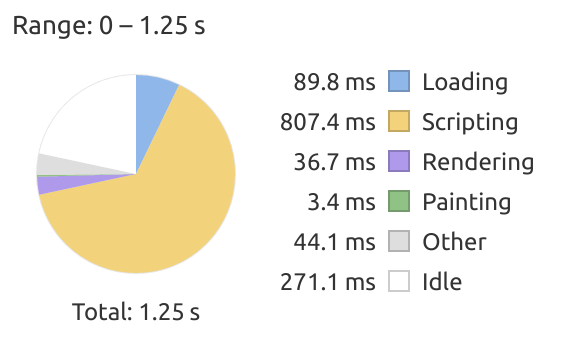
\includegraphics[width=\textwidth]{figure/clientsidePerformance/graph1.png}
    \end{subfigure}
    \begin{subfigure}{0.49\textwidth}
        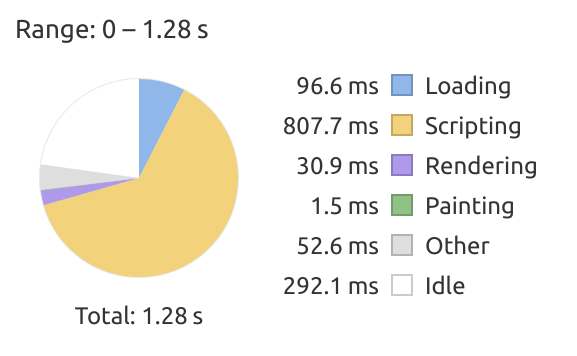
\includegraphics[width=\textwidth]{figure/clientsidePerformance/graph2.png}
    \end{subfigure}
    \\
    \begin{subfigure}{0.5\textwidth}
        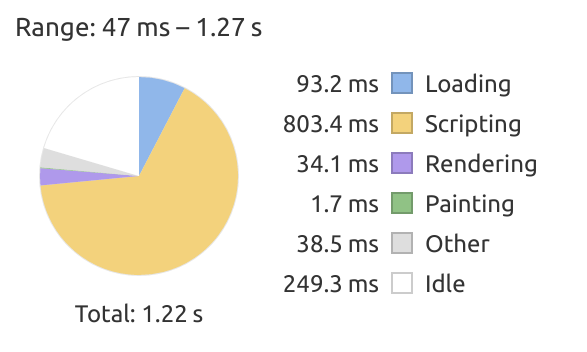
\includegraphics[width=\textwidth]{figure/clientsidePerformance/graph3.png}
    \end{subfigure}
    
    \caption{Loading the clientside javascript on our application with no games and 1 player connected.}
    %\label{fig:my_label}
\end{figure}

\begin{figure}[H]
    \centering
    \begin{subfigure}{0.49\textwidth}
        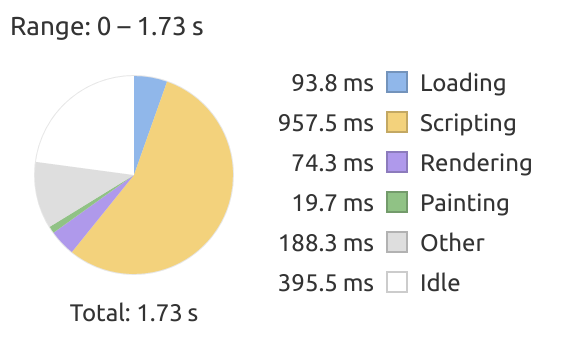
\includegraphics[width=\textwidth]{figure/clientsidePerformance/graph30games1.png}
    \end{subfigure}
    \begin{subfigure}{0.49\textwidth}
        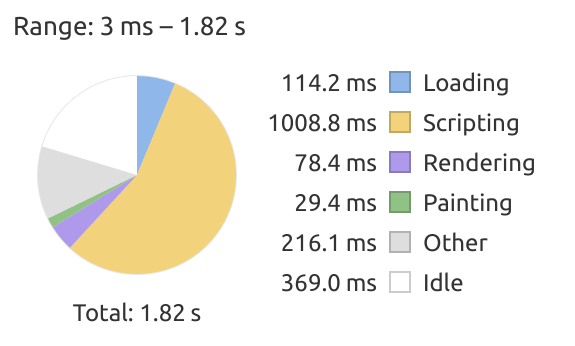
\includegraphics[width=\textwidth]{figure/clientsidePerformance/graph30games2.png}
    \end{subfigure}
    \\
    \begin{subfigure}{0.5\textwidth}
        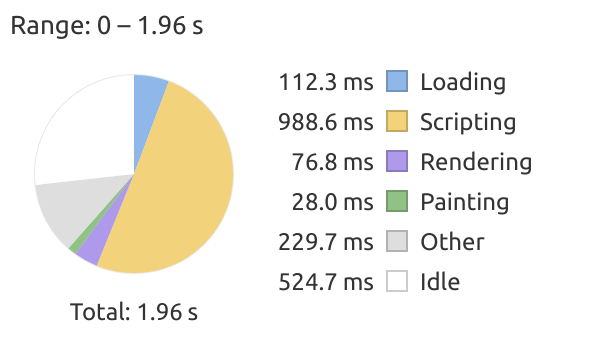
\includegraphics[width=\textwidth]{figure/clientsidePerformance/graph30games3.png}
    \end{subfigure}
    
    \caption{Loading the clientside javascript on our application with 30 games and 1 player connected.}
    %\label{fig:my_label}
\end{figure}

\begin{figure}[H]
    \centering
    \begin{subfigure}{0.49\textwidth}
        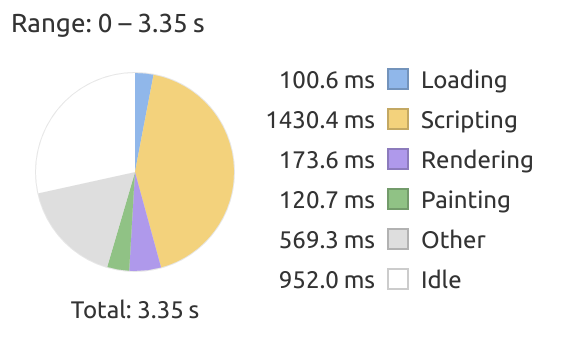
\includegraphics[width=\textwidth]{figure/clientsidePerformance/graph90games1.png}
    \end{subfigure}
    \begin{subfigure}{0.49\textwidth}
        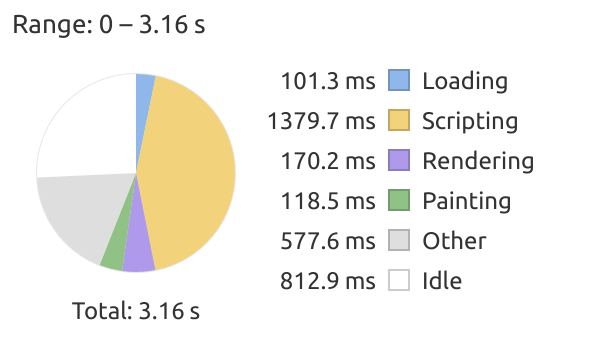
\includegraphics[width=\textwidth]{figure/clientsidePerformance/graph90games2.png}
    \end{subfigure}
    \\
    \begin{subfigure}{0.5\textwidth}
        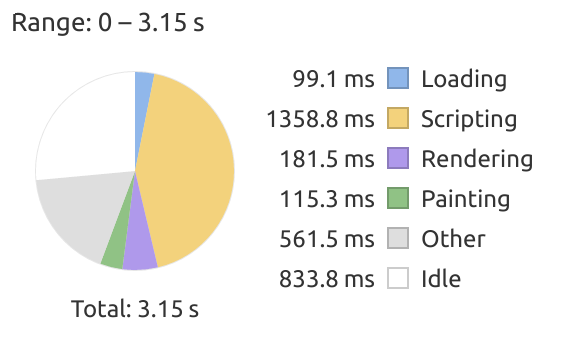
\includegraphics[width=\textwidth]{figure/clientsidePerformance/graph90games3.png}
    \end{subfigure}
    
    \caption{Loading the clientside javascript on our application with 90 games and 1 player connected.}
    %\label{fig:my_label}
\end{figure}

\begin{figure}[H]
    \centering
    \begin{subfigure}{0.49\textwidth}
        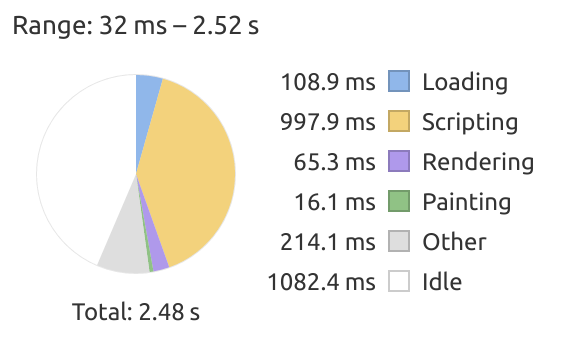
\includegraphics[width=\textwidth]{figure/clientsidePerformance/braseegraph1.png}
    \end{subfigure}
    \begin{subfigure}{0.49\textwidth}
        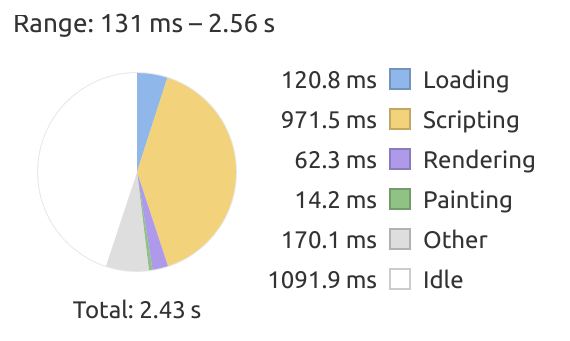
\includegraphics[width=\textwidth]{figure/clientsidePerformance/braseegraph2.png}
    \end{subfigure}
    \\
    \begin{subfigure}{0.5\textwidth}
        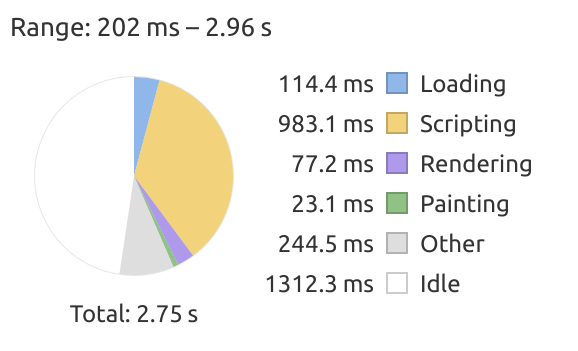
\includegraphics[width=\textwidth]{figure/clientsidePerformance/braseegraph3.png}
    \end{subfigure}
    
    \caption{Loading brasee.com lobby with approximately 10 players and 3 games.}
    %\label{fig:my_label}
\end{figure}

\begin{figure}[H]
    \centering
    \begin{subfigure}{0.49\textwidth}
        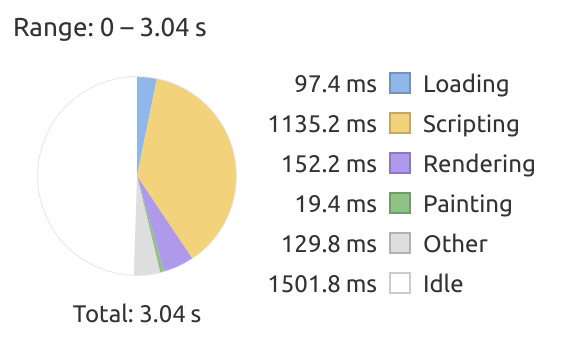
\includegraphics[width=\textwidth]{figure/clientsidePerformance/ligraph1.png}
    \end{subfigure}
    \begin{subfigure}{0.49\textwidth}
        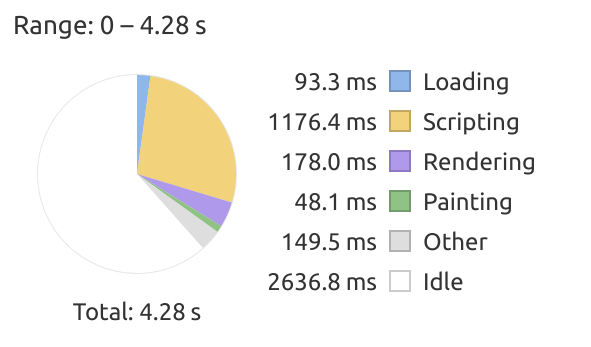
\includegraphics[width=\textwidth]{figure/clientsidePerformance/ligraph2.png}
    \end{subfigure}
    \\
    \begin{subfigure}{0.5\textwidth}
        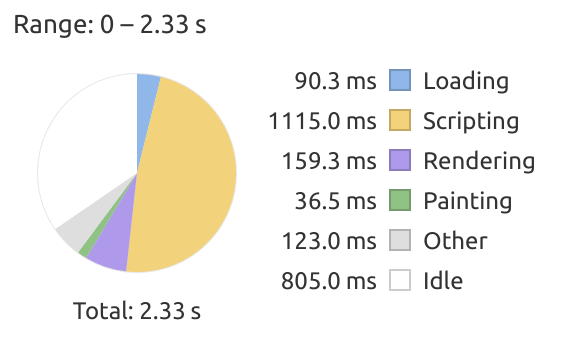
\includegraphics[width=\textwidth]{figure/clientsidePerformance/ligraph3.png}
    \end{subfigure}
    
    \caption{Loading lichess.org with approximately 6000 players and 1500 games.}
    %\label{fig:my_label}
\end{figure}
\newpage

\subsection{Performance test of the server application}
\begin{figure}[H]
    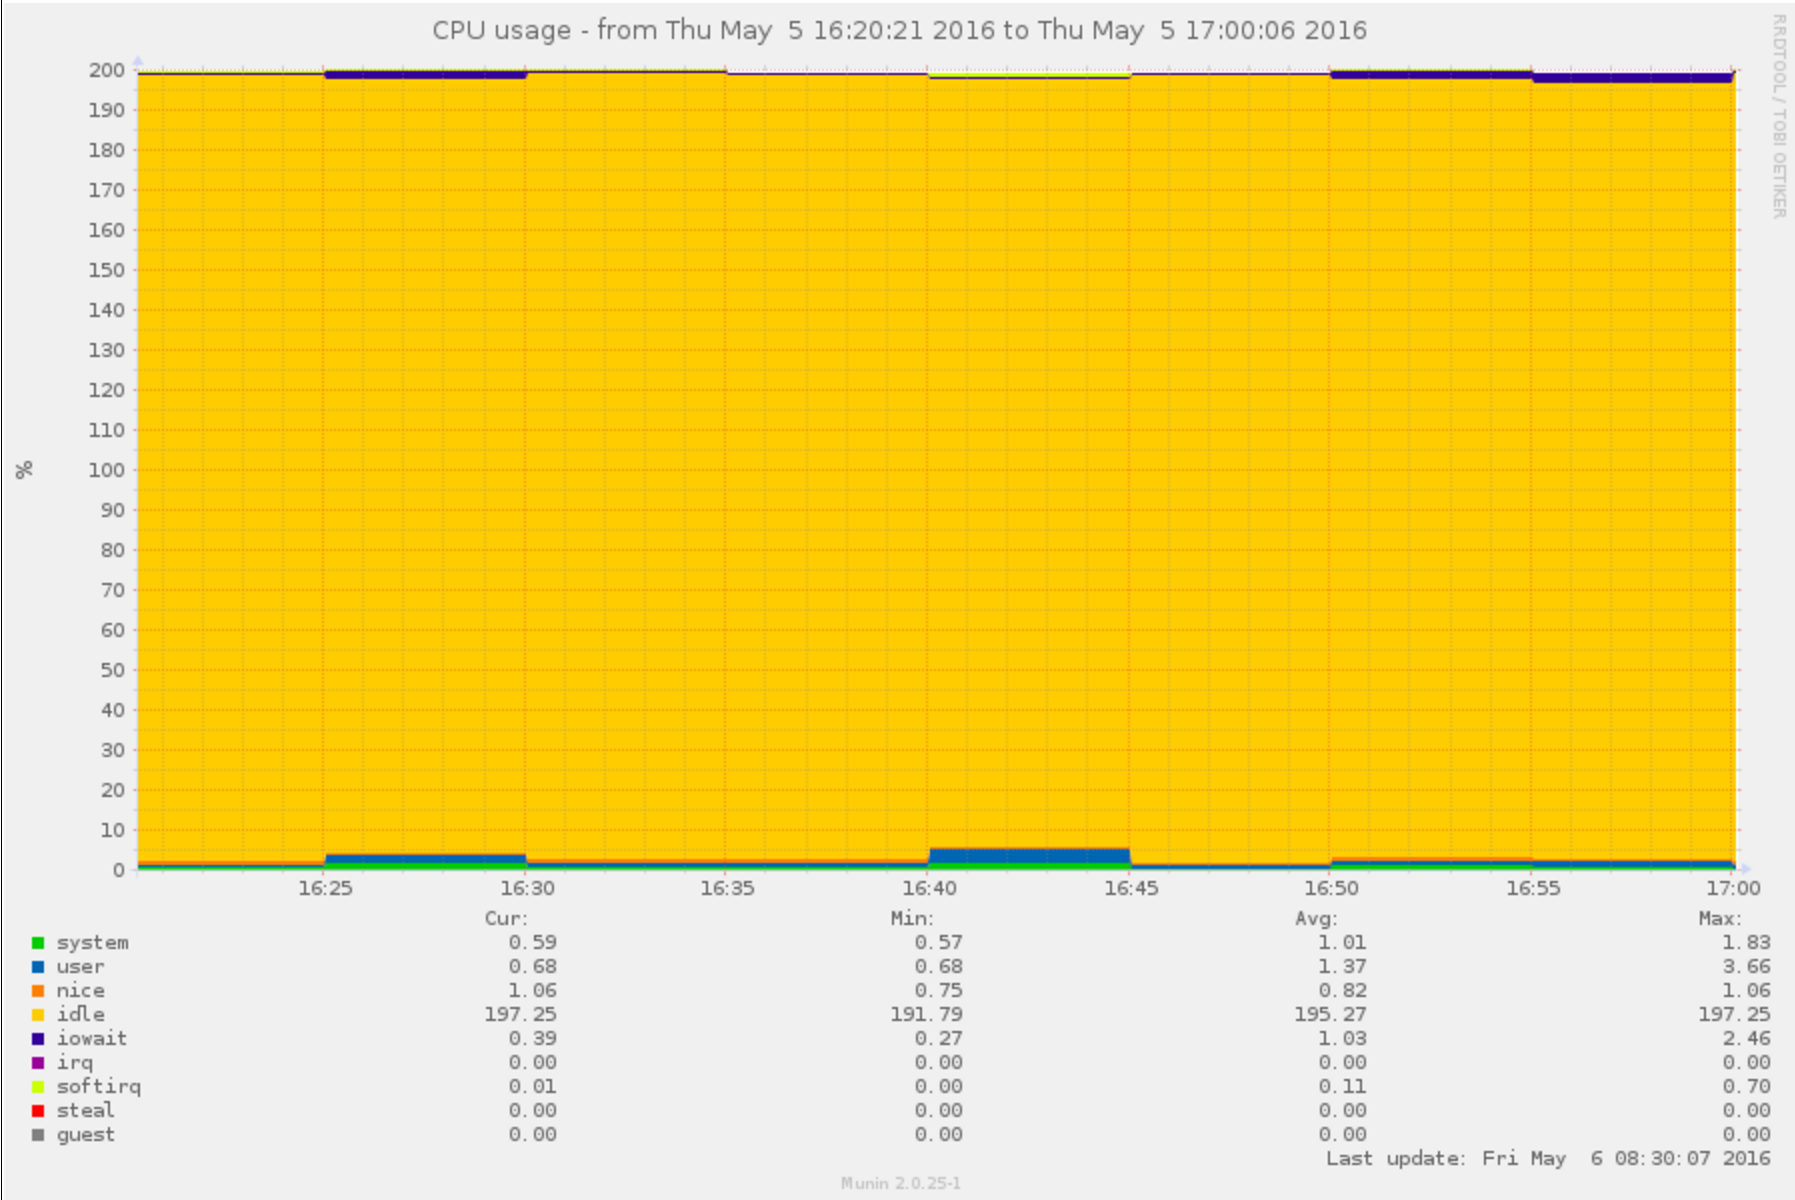
\includegraphics[width=0.95\textwidth]{figure/serversidePerformance/2016-05-05-chatting-test-cpu.png}
    \caption{CPU usage during the chat test}
    \label{fig:cpu-results-attachment}
\end{figure}

\begin{figure}[H]
    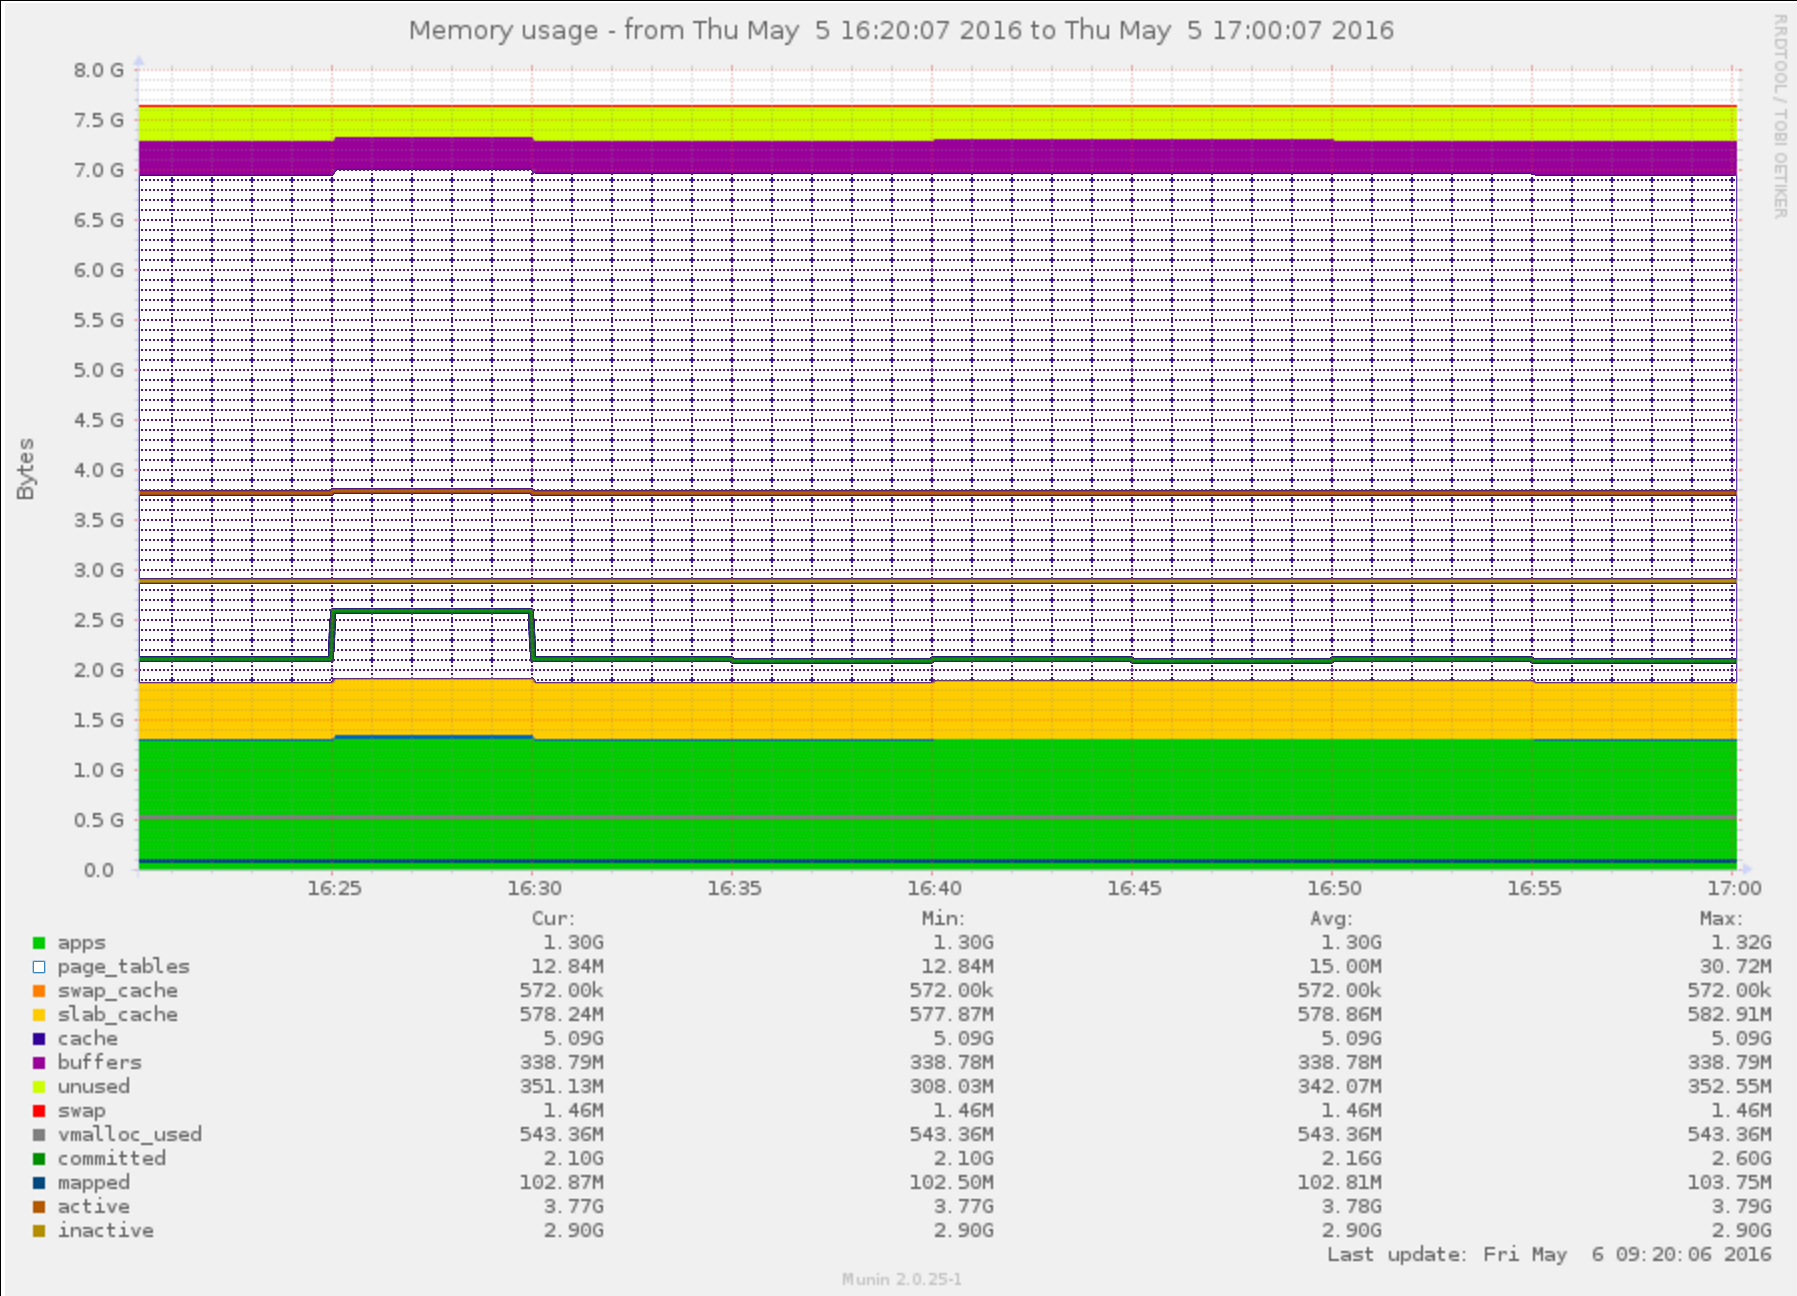
\includegraphics[width=\textwidth]{figure/serversidePerformance/2016-05-05-chat-memory.png}
    \caption{Memory usage on the server during the chat test}
    \label{fig:memory-results-attachment}
\end{figure}


\begin{figure}[H]
    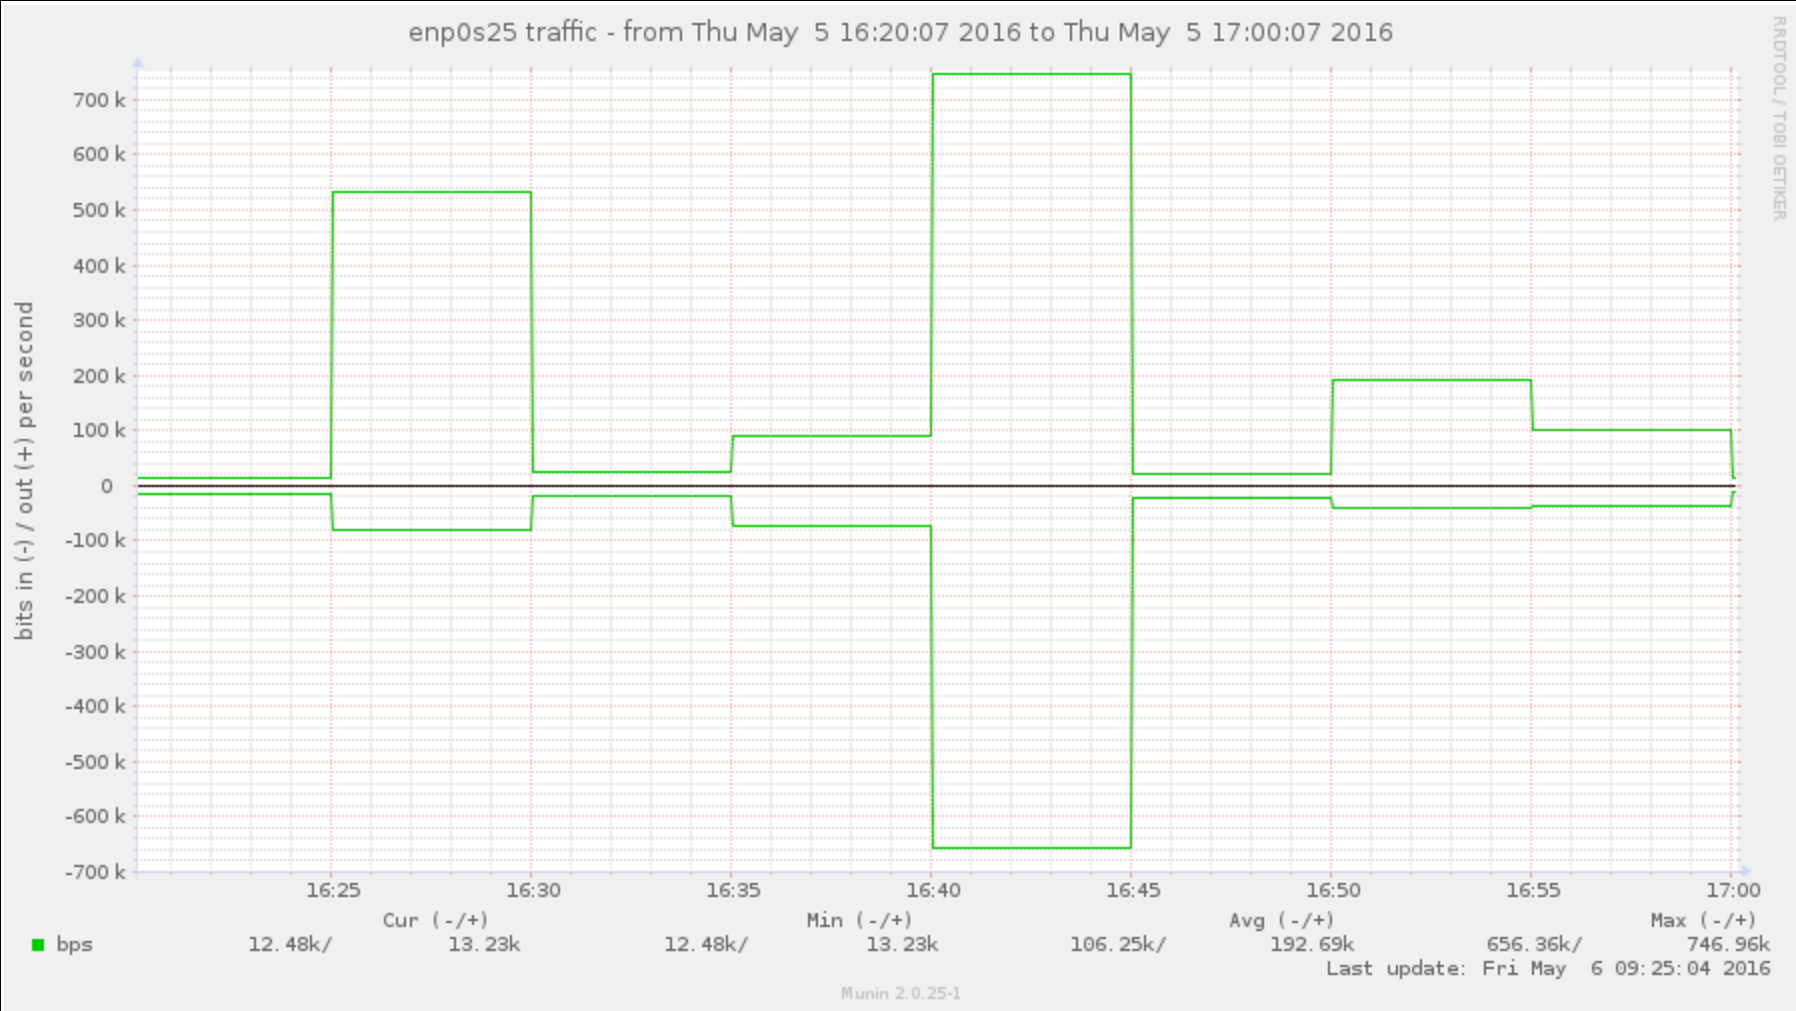
\includegraphics[width=\textwidth]{figure/serversidePerformance/2016-05-05-network-traffic-chat.png}
    \caption{Network traffic on the server during the chat test}
    \label{fig:network-results-attachment}
\end{figure}

\begin{figure}[H]
    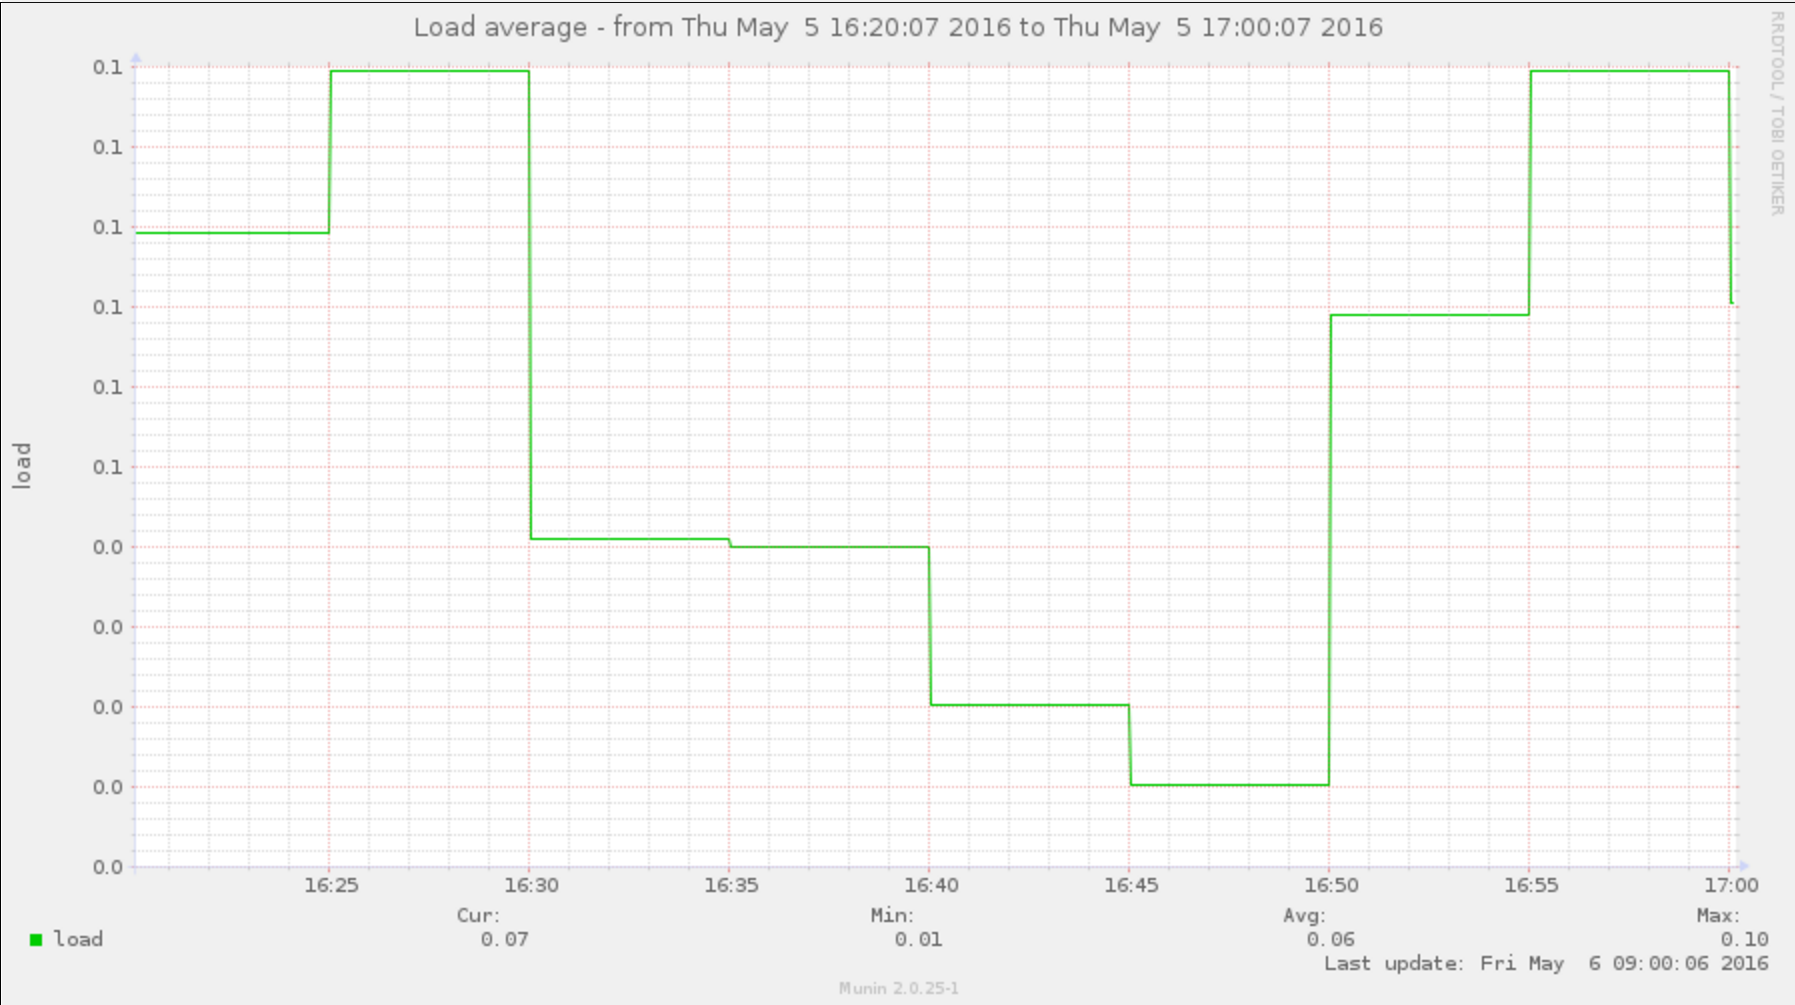
\includegraphics[width=\textwidth]{figure/serversidePerformance/2016-05-05-load-average-chatting-tests.png}
    \caption{Load average on the server during the chat test}
    \label{fig:load-average-results-attachment}
\end{figure}


\end{document}
